\documentclass[11pt]{article}

\usepackage{graphicx}
\usepackage{listings}
\usepackage{url}
\usepackage{float} % Add this package for the [H] option
\usepackage{listings}
\usepackage{color}

\definecolor{dkgreen}{rgb}{0,0.6,0}
\definecolor{gray}{rgb}{0.5,0.5,0.5}
\definecolor{mauve}{rgb}{0.58,0,0.82}
\usepackage{minted}

\lstset{frame=tb,
  language=Java,
  aboveskip=3mm,
  belowskip=3mm,
  showstringspaces=false,
  columns=flexible,
  basicstyle={\small\ttfamily},
  numbers=none,
  numberstyle=\tiny\color{gray},
  keywordstyle=\color{blue},
  commentstyle=\color{dkgreen},
  stringstyle=\color{mauve},
  breaklines=true,
  breakatwhitespace=true,
  tabsize=3
}

\begin{document}

\begin{titlepage}
    \begin{center}
        
\includegraphics[scale=0.10]{du.png}\par
        \begin{Huge}
            \textsc{University of Dhaka}\par
        \end{Huge}
        \begin{Large}
            Department of Computer Science and Engineering\par \vspace{1cm}
            CSE-3111 : Computer Networking Lab \\[12pt]   
            Lab Report 4 : Distributed Database Management,\\[8pt]Implementation of Iterative, and Recursive
Queries of \\[8pt]DNS Records.
        \end{Large}
    \end{center}     
    \begin{large}
        \textbf{Submitted By:\\[12pt]}
            Name: Md Shamsur Rahman Sami\\[5pt]
            Roll No : 57\\[7pt]
            Name: Md Rakib Hossain\\[5pt]
            Roll No : 55\\[12pt]
        \textbf{Submitted On : \\[12pt]}
            February 15, 2024\\[20pt]
        \textbf{Submitted To :\\[12pt]}
            Dr. Md. Abdur Razzaque\\[12pt]
    \end{large}
\end{titlepage}

\tableofcontents  

\newpage

\section{Introduction}
\subsection{Objectives}

The primary objective of this lab is to provide students with comprehensive hands-on experience in the setup and management of a Domain Name System (DNS) server, coupled with the implementation and comparison of iterative and recursive DNS resolution methods. Through practical exercises, participants will delve into the intricacies of configuring a DNS server, creating and managing DNS records, and subsequently developing scripts or programs to execute DNS queries. By scrutinizing the performance metrics and intricacies of iterative versus recursive resolution techniques across various scenarios, students will gain a nuanced understanding of DNS operation efficiency, while also discerning the distinct advantages, disadvantages, and security ramifications inherent to each method.

\section{Theory of Distributed Database Management and DNS Queries}

This section provides a theoretical overview of distributed database management systems (DDBMS) and the implementation of iterative and recursive queries for DNS (Domain Name System) records.

\subsection{Distributed Database Management}

\begin{itemize}
\item \textbf{Concepts:} Distributed database management involves the storage and management of data across multiple interconnected nodes or locations.
\item \textbf{Advantages:} DDBMS offers benefits such as improved data availability, scalability, fault tolerance, and better performance through data replication and distribution.
\item \textbf{Architecture:} DDBMS typically comprises distributed database servers, network infrastructure, and middleware for communication and coordination.
\end{itemize}

\subsection{DNS (Domain Name System)}

\begin{itemize}
\item \textbf{Functionality:} DNS is a hierarchical decentralized naming system that translates domain names into IP addresses, facilitating the navigation of the internet.
\item \textbf{Records:} DNS records contain information mapping domain names to IP addresses (A records), mail servers (MX records), aliases (CNAME records), and other resource records.
\item \textbf{Resolution Process:} DNS resolution involves iterative or recursive queries to DNS servers to obtain IP addresses associated with domain names.
\end{itemize}

\subsection{Implementation of Iterative DNS Queries}

\begin{itemize}
\item \textbf{Iterative Query Process:} In iterative DNS resolution, a DNS client sends queries to DNS servers sequentially, and each server responds with the best information it has or refers the client to another server.
\item \textbf{Implementation Steps:} Implementing iterative DNS queries involves sending queries to DNS servers, processing responses, and following referrals until the desired IP address is obtained or a timeout occurs.
\end{itemize}

\subsection{Implementation of Recursive DNS Queries}

\begin{itemize}
\item \textbf{Recursive Query Process:} In recursive DNS resolution, a DNS client sends a query to a DNS server, which then recursively queries other servers on behalf of the client until it obtains the IP address or determines it does not exist.
\item \textbf{Implementation Steps:} Implementing recursive DNS queries requires a DNS server capable of recursively querying other DNS servers, processing responses, and caching results to improve performance.
\end{itemize}

\subsection{Comparison of Iterative and Recursive Queries}

\begin{itemize}
\item \textbf{Efficiency:} Iterative queries may involve multiple round-trip communications but provide more control over the resolution process. Recursive queries delegate resolution to DNS servers but may incur higher latency.
\item \textbf{Scalability:} Recursive queries offload resolution tasks to DNS servers, making them suitable for large-scale environments. Iterative queries distribute workload to clients but may overwhelm servers with frequent queries.
\end{itemize}

\subsection{Security Considerations}

\begin{itemize}
\item \textbf{Cache Poisoning:} Both iterative and recursive DNS resolution methods are vulnerable to cache poisoning attacks, where malicious data is inserted into DNS caches to redirect traffic.
\item \textbf{Encryption:} Implementing DNS over HTTPS (DoH) or DNS over TLS (DoT) can enhance security by encrypting DNS traffic and preventing eavesdropping or tampering.
\end{itemize}

\section{Methodology}

This section outlines the methodology followed to conduct the lab experiment on distributed database management and the implementation of iterative and recursive queries for DNS records.

\subsection{Setup and Configuration}

\begin{enumerate}
\item \textbf{Environment Setup:} Configure a network environment comprising multiple machines to simulate distributed database management and DNS resolution scenarios.
\item \textbf{Database Setup:} Install and configure distributed database management software (e.g., MySQL Cluster, Apache Cassandra) on designated server nodes to create distributed database instances.
\item \textbf{DNS Server Setup:} Set up a DNS server (e.g., BIND, dnsmasq) on a separate server node to handle DNS queries and host DNS records for domain resolution.
\end{enumerate}

\subsection{Experiment Design}

\begin{enumerate}
\item \textbf{Database Experiment:} Design experiments to assess the performance and scalability of distributed database management systems. Consider factors such as data distribution, replication strategies, query processing, and fault tolerance mechanisms.
\item \textbf{DNS Query Experiment:} Define experiments to evaluate the effectiveness and efficiency of iterative and recursive DNS queries. Vary parameters such as query types, domain names, DNS server configurations, and network conditions.
\end{enumerate}

\subsection{Implementation of Iterative DNS Queries}

\begin{enumerate}
\item \textbf{Programming Language Selection:} Choose a suitable programming language with robust networking capabilities - Python for implementing iterative DNS query scripts.
\item \textbf{Socket Programming:} Utilize the socket API to create client-side scripts that send iterative DNS queries to DNS servers and process responses sequentially.
\item \textbf{Error Handling:} Implement error handling mechanisms to handle connection timeouts, DNS server unavailability, and other network-related issues during iterative query execution.
\end{enumerate}

\subsection{Implementation of Recursive DNS Queries}

\begin{enumerate}
\item \textbf{DNS Server Configuration:} Configure the DNS server to support recursive queries and enable caching to improve query resolution performance.
\item \textbf{Client-Side Scripting:} Develop client-side scripts using a suitable programming language to send recursive DNS queries to the DNS server and handle responses.
\item \textbf{Caching Mechanism:} Implement caching mechanisms in the client script to store resolved DNS records and optimize subsequent query resolutions.
\end{enumerate}

\subsection{Experiment Execution}

\begin{enumerate}
\item \textbf{Database Experiment:} Execute experiments on the distributed database setup to measure performance metrics such as query latency, throughput, scalability, and fault tolerance under varying loads and configurations.
\item \textbf{DNS Query Experiment:} Conduct experiments to compare the performance of iterative and recursive DNS queries in terms of query resolution time, network overhead, and scalability across different scenarios.
\end{enumerate}

\subsection{Data Collection and Analysis}

\begin{enumerate}
\item \textbf{Database Experiment Data:} Collect experimental data including query execution times, throughput, and system resource utilization metrics from the distributed database environment.
\item \textbf{DNS Query Experiment Data:} Gather data on DNS query resolution times, network traffic, and server load for both iterative and recursive query methods.
\item \textbf{Analysis:} Analyze collected data to evaluate the effectiveness, efficiency, and scalability of distributed database management systems and DNS query resolution methods. Compare results to draw conclusions and identify any performance bottlenecks or areas for improvement.
\end{enumerate}

\subsection{Reporting}

\begin{enumerate}
\item \textbf{Documentation:} Document experimental setup details, methodology, results, and analysis in a comprehensive lab report.
\item \textbf{Presentation:} Prepare a presentation summarizing the lab experiment, key findings, and conclusions for presentation to peers or instructors.
\end{enumerate}





\section{Experimental Result}

\subsection{Task 1}


\begin{itemize}
    \item \textbf{Setting up the DNS server}
    
    
    \begin{minted}[mathescape, linenos]{python}
    SERVER SIDE CODE
   
import socket

class IPSearch:
    list = []

    def create_list():
        ins = IPSearch("cse.du.ac.bd.", "ns1.cse.du.ac.bd.", "NS", "86400")
        IPSearch.list.append(ins)
        ins3 = IPSearch("ns2.cse.du.ac.bd.", "192.0.2.2", "A", "86400")
        IPSearch.list.append(ins3)
        ins4 = IPSearch("ns1.cse.du.ac.bd.", "2001:db8::1", "AAAA", "86400")
        IPSearch.list.append(ins4)
        ins5 = IPSearch("ns2.cse.du.ac.bd.", "2001:db8::2", "AAAA", "86400")
        IPSearch.list.append(ins5)
        ins6 = IPSearch("cse.du.ac.bd.", "192.0.2.3", "A", "86400")
        IPSearch.list.append(ins6)
        ins7 = IPSearch("cse1.du.ac.bd.", "2001:db8::3", "AAAA", "86400")
        IPSearch.list.append(ins7)
        ins8 = IPSearch("www.cse.du.ac.bd.", "cse.du.ac.bd.", "CNAME", "86400")
        IPSearch.list.append(ins8)
        ins9 = IPSearch("cse2.du.ac.bd.", "10 mail.cse.du.ac.bd.", "MX", "86400")
        IPSearch.list.append(ins9)
        ins10 = IPSearch("mail.cse.du.ac.bd.", "192.0.2.4", "A", "86400")
        IPSearch.list.append(ins10)
        

    def __init__(self, Name, Value, Type, TTL):
        self.Name = Name
        self.Value = Value
        self.Type = Type
        self.TTL = TTL

class Server:
    def search(s):
        ret = 0
        rs = "nf"
        for item in IPSearch.list:
            if item.Name == s:
                rs = item.Type
                break

        if rs.strip() == "NS":
            return 1
        elif rs.strip() == "MX":
            return 5
        elif rs.strip() == "nf":
            return 0
        elif rs.strip() == "CNAME":
            return 2
        elif rs.strip() == "AAAA":
            return 3
        elif rs.strip() == "A":
            return 4
        return ret
    

    # def search1(s):
    #     ret = 0
    #     rs = "nf"
    #     for item in IPSearch.list:
    #         if item.Name == s:
    #             rs = item.Type
    #             break

    #     if rs.strip() == "NS":
    #         return 1
    #     elif rs.strip() == "MX":
    #         return 5
    #     elif rs.strip() == "nf":
    #         return 0
    #     elif rs.strip() == "CNAME":
    #         return 2
    #     elif rs.strip() == "AAAA":
    #         return 3
    #     elif rs.strip() == "A":
    #         return 4
    #     return ret

    def main():
        IPSearch.create_list()
        response = "Welcome to CSE 3111!"
        port = 1500
        server_socket = socket.socket(socket.AF_INET, socket.SOCK_DGRAM)
        server_socket.bind((socket.gethostname(), port))
        print("Domain server Started")
        buffer_size = 1024

        while True:
            buffer, client_address = server_socket.recvfrom(buffer_size)
            message = buffer.decode().strip()
            print("Client message:", message)
            flag = Server.search(message)
            print(flag)

            if flag == 0:
                response = "Not Found"
            elif flag == 1:
                response = "NS type domain found"
            elif flag == 2:
                response = "Cname type domain found"
            elif flag == 3:
                response = "AAAA type domain found"
            elif flag == 4:
                response = "A type domain found"
                # response = IPSearch.list[IPSearch.index].Value
            elif flag == 5:
                response = "MX type domain found"

            server_socket.sendto(response.encode(), client_address)

        server_socket.close()

if __name__ == "__main__":
    Server.main()


\end{minted}


    \begin{minted}[mathescape, linenos]{python}
    CLIENT SIDE CODE
import socket

def string_to_binary(input_string):
    binary_representation = ' '.join(format(ord(char), '08b') for char in input_string)
    return binary_representation



udp_socket = socket.socket(socket.AF_INET, socket.SOCK_DGRAM)
message = "mail.cse.du.ac.bd."

buffer = message.encode('utf-8')
server_address = ('10.42.0.74', 1500)


udp_socket.sendto(buffer, server_address)

buffer, server_address = udp_socket.recvfrom(1024)
response = buffer.decode('utf-8')

binary_result = string_to_binary(response)
print(f"Server Response : After Encode : {binary_result}")


print("Server response: After Decode : ", response)

udp_socket.close()
    
\end{minted}
    \begin{figure}[H]
        \centering
        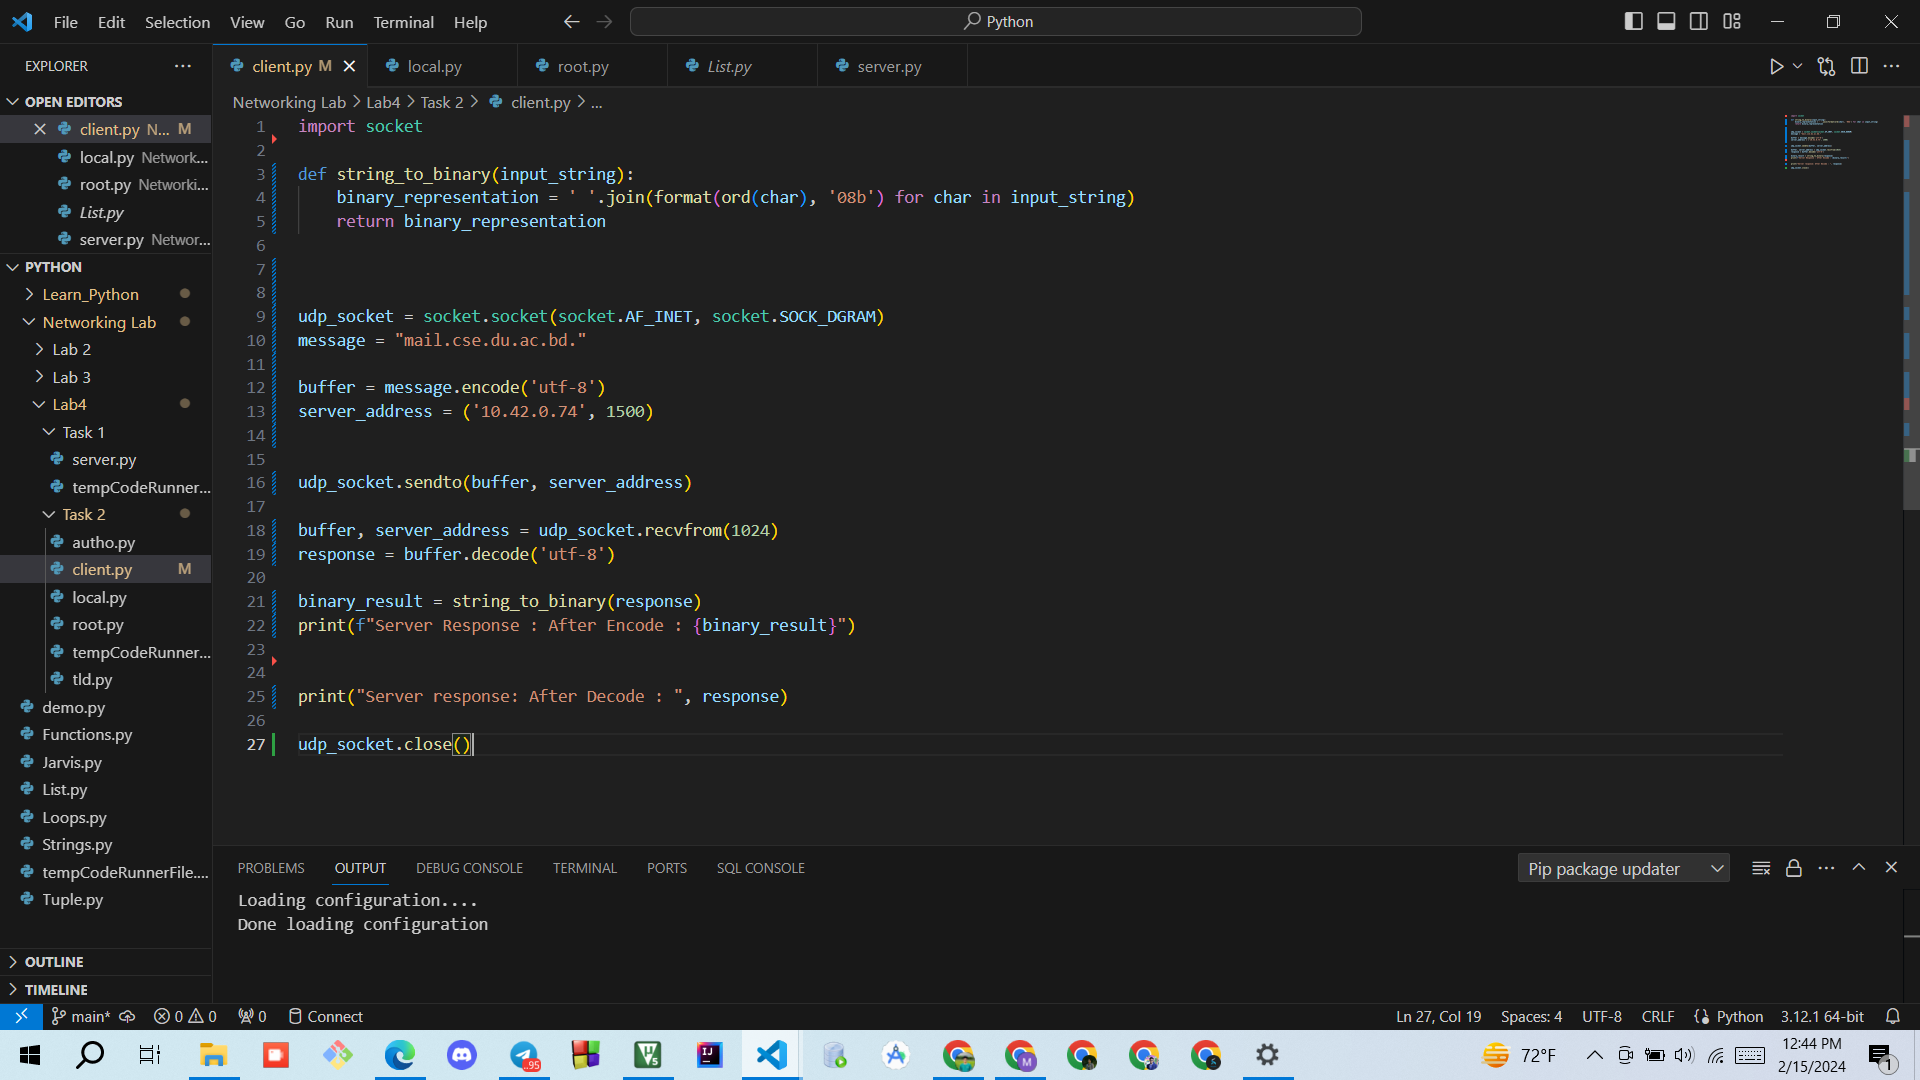
\includegraphics[width=0.8\textwidth]{Screenshot (163).png}
        \caption{Client side code}
        \label{fig:1}
    \end{figure}
    
    \begin{figure}[H]
        \centering
        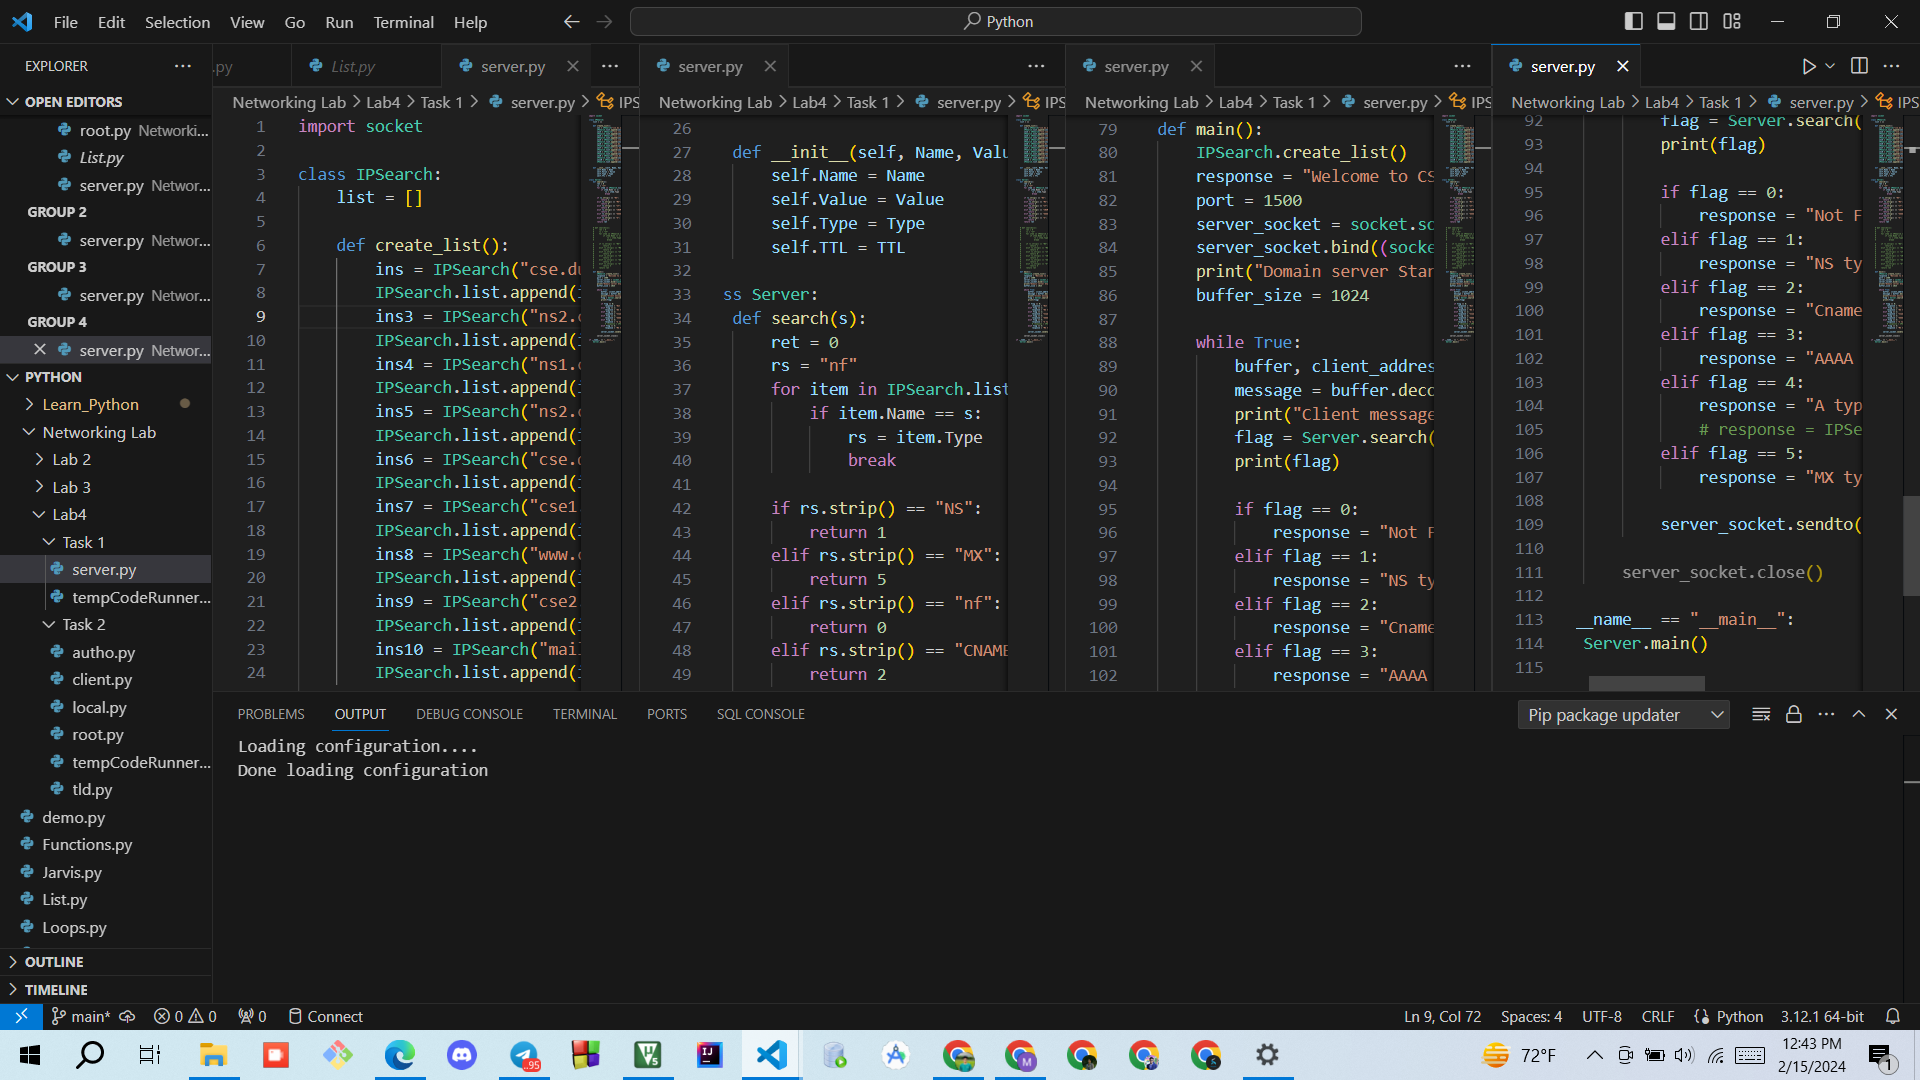
\includegraphics[width=0.8\textwidth]{Screenshot (161).png}
        \caption{Server Side Code}
        \label{fig:2}
    \end{figure}
    
    

\end{itemize}

 
\subsection{Task 2}
\begin{itemize}
\item \textbf{Iterative DNS resolution.}
    \begin{minted}[mathescape, linenos]{python}
    Local SERVER SIDE CODE
    
import socket
import struct

def main():
    # Create a UDP socket
    socket_server = socket.socket(socket.AF_INET, socket.SOCK_DGRAM)
    socket_server.bind(('localhost', 5000))

    while True:
        # Receive message from client
        receive_data, address = socket_server.recvfrom(1024)
        message_length = struct.unpack('!I', receive_data[:4])[0]
        domain = receive_data[4:4+message_length].decode('utf-8')
        print("Received from client:", domain)

        # Send message to Root DNS Server
        root_dns_address = ('localhost', 7000)
        send_message(socket_server, root_dns_address, domain)

        # Receive message from Root DNS Server
        root_dns_response = receive_message(socket_server)

        # Send message to TLD DNS Server
        tld_dns_address = ('localhost', 9876)
        send_message(socket_server, tld_dns_address, "0.0.0.1")

        # Receive message from TLD DNS Server
        tld_dns_response = receive_message(socket_server)

        # Send message to Authoritative DNS Server
        auth_dns_address = ('localhost', 9000)
        send_message(socket_server, auth_dns_address, "0.0.1.0")

        # Receive message from Authoritative DNS Server
        auth_dns_response = receive_message(socket_server)

        # Send message back to client
        #client_address = (address[0], 5000)
        send_message(socket_server, address, "0.0.1.0")

    socket_server.close()

def send_message(socket_server, address, ip):
    message_bytes = ip.encode('utf-8')
    message_length = len(message_bytes)
    buffer = struct.pack('!HBBI', 1, 2, 2, message_length) + message_bytes
    print("Sending to", address[0] + ":", ip)
    socket_server.sendto(buffer, address)

def receive_message(socket_server):
    receive_data, address = socket_server.recvfrom(1024)
    message_length = struct.unpack('!I', receive_data[:4])[0]
    ip = receive_data[4:4+message_length].decode('utf-8')
    print("Received from", address[0] + ":", ip)
    return ip

if __name__ == "__main__":
    main()


\end{minted}
  
  \begin{minted}[mathescape, linenos]{python}
    Root SERVER SIDE CODE
    
import socket
import struct

def main():
    # Create a UDP socket
    socket_server = socket.socket(socket.AF_INET, socket.SOCK_DGRAM)
    socket_server.bind(('localhost', 7000))

    # Receive message from Local DNS Server
    receive_data, address = socket_server.recvfrom(1024)
    message_length = struct.unpack('!I', receive_data[:4])[0]
    domain = receive_data[4:4+message_length].decode('utf-8')
    print("Received from Local DNS:", domain)

    # Sending message to Local DNS Server
    IP = "0.0.0.1"
    message_bytes = IP.encode('utf-8')
    message_length = len(message_bytes)

    buffer = struct.pack('!HBBI', 1, 2, 2, message_length) + message_bytes

    print("Sending to Local DNS:", IP)
    socket_server.sendto(buffer, ('localhost', 5000))

    socket_server.close()

if __name__ == "__main__":
    main()

\end{minted}
  \begin{minted}[mathescape, linenos]{python}
    TLD SERVER SIDE CODE
    
import socket
import struct

def main():
    # Create a UDP socket
    socket_server = socket.socket(socket.AF_INET, socket.SOCK_DGRAM)
    socket_server.bind(('localhost', 9876))

    while True:
        # Receive message from Local DNS Server
        receive_data, address = socket_server.recvfrom(1024)
        message_length = struct.unpack('!I', receive_data[:4])[0]
        domain = receive_data[4:4+message_length].decode('utf-8')
        print("Receiving from local DNS:", domain)

        # Send message from Local DNS Server
        IP = "0.0.1.0"
        send_message(socket_server, ('localhost', 5000), IP)

    socket_server.close()

def send_message(socket_server, address, ip):
    message_bytes = ip.encode('utf-8')
    message_length = len(message_bytes)
    buffer = struct.pack('!HBBI', 1, 2, 2, message_length) + message_bytes
    print("Sending to Local DNS:", ip)
    socket_server.sendto(buffer, address)

if __name__ == "__main__":
    main()


\end{minted}
\begin{minted}[mathescape, linenos]{python}
    Authorititive SERVER SIDE CODE
    
import socket
import struct

def main():
    # Create a UDP socket
    socket_server = socket.socket(socket.AF_INET, socket.SOCK_DGRAM)
    socket_server.bind(('localhost', 9000))

    while True:
        # Receive message from Local DNS Server
        receive_data, address = socket_server.recvfrom(1024)
        message_length = struct.unpack('!I', receive_data[:4])[0]
        domain = receive_data[4:4+message_length].decode('utf-8')
        print("Receiving from local DNS:", domain)

        # Send message from Local DNS Server
        IP = "1.0.2.1"
        send_message(socket_server, ('localhost', 5000), IP)

    socket_server.close()

def send_message(socket_server, address, ip):
    message_bytes = ip.encode('utf-8')
    message_length = len(message_bytes)
    buffer = struct.pack('!HBBI', 1, 2, 2, message_length) + message_bytes
    print("Sending to Local DNS:", ip)
    socket_server.sendto(buffer, address)

if __name__ == "__main__":
    main()


\end{minted}
    \begin{minted}[mathescape, linenos]{python}
    CLIENT SIDE CODE
  import socket
import struct

def main():
    socket_client = socket.socket(socket.AF_INET, socket.SOCK_DGRAM)
    server_address = ('localhost', 5000)

    # Sending Domain to Local DNS Server
    domain = "www.cse.du.ac.bd"
    print("Sent Domain:", domain)
    message_bytes = domain.encode('utf-8')
    message_length = len(message_bytes)

    # Packing data into byte array
    send_data = struct.pack("!HBBi", 1, 2, 2, message_length) + message_bytes

    socket_client.sendto(send_data, server_address)

    # Receiving IP from the Local DNS Server
    receive_data, server = socket_client.recvfrom(1024)
    message_length, = struct.unpack("!i", receive_data[:4])
    IP = receive_data[4:message_length + 4].decode('utf-8')
    print("Received IP:", IP)

    socket_client.close()

if __name__ == "__main__":
    main()

\end{minted}

\begin{itemize}
    \item \textbf{}
    
  . 
    \begin{figure}[H]
        \centering
        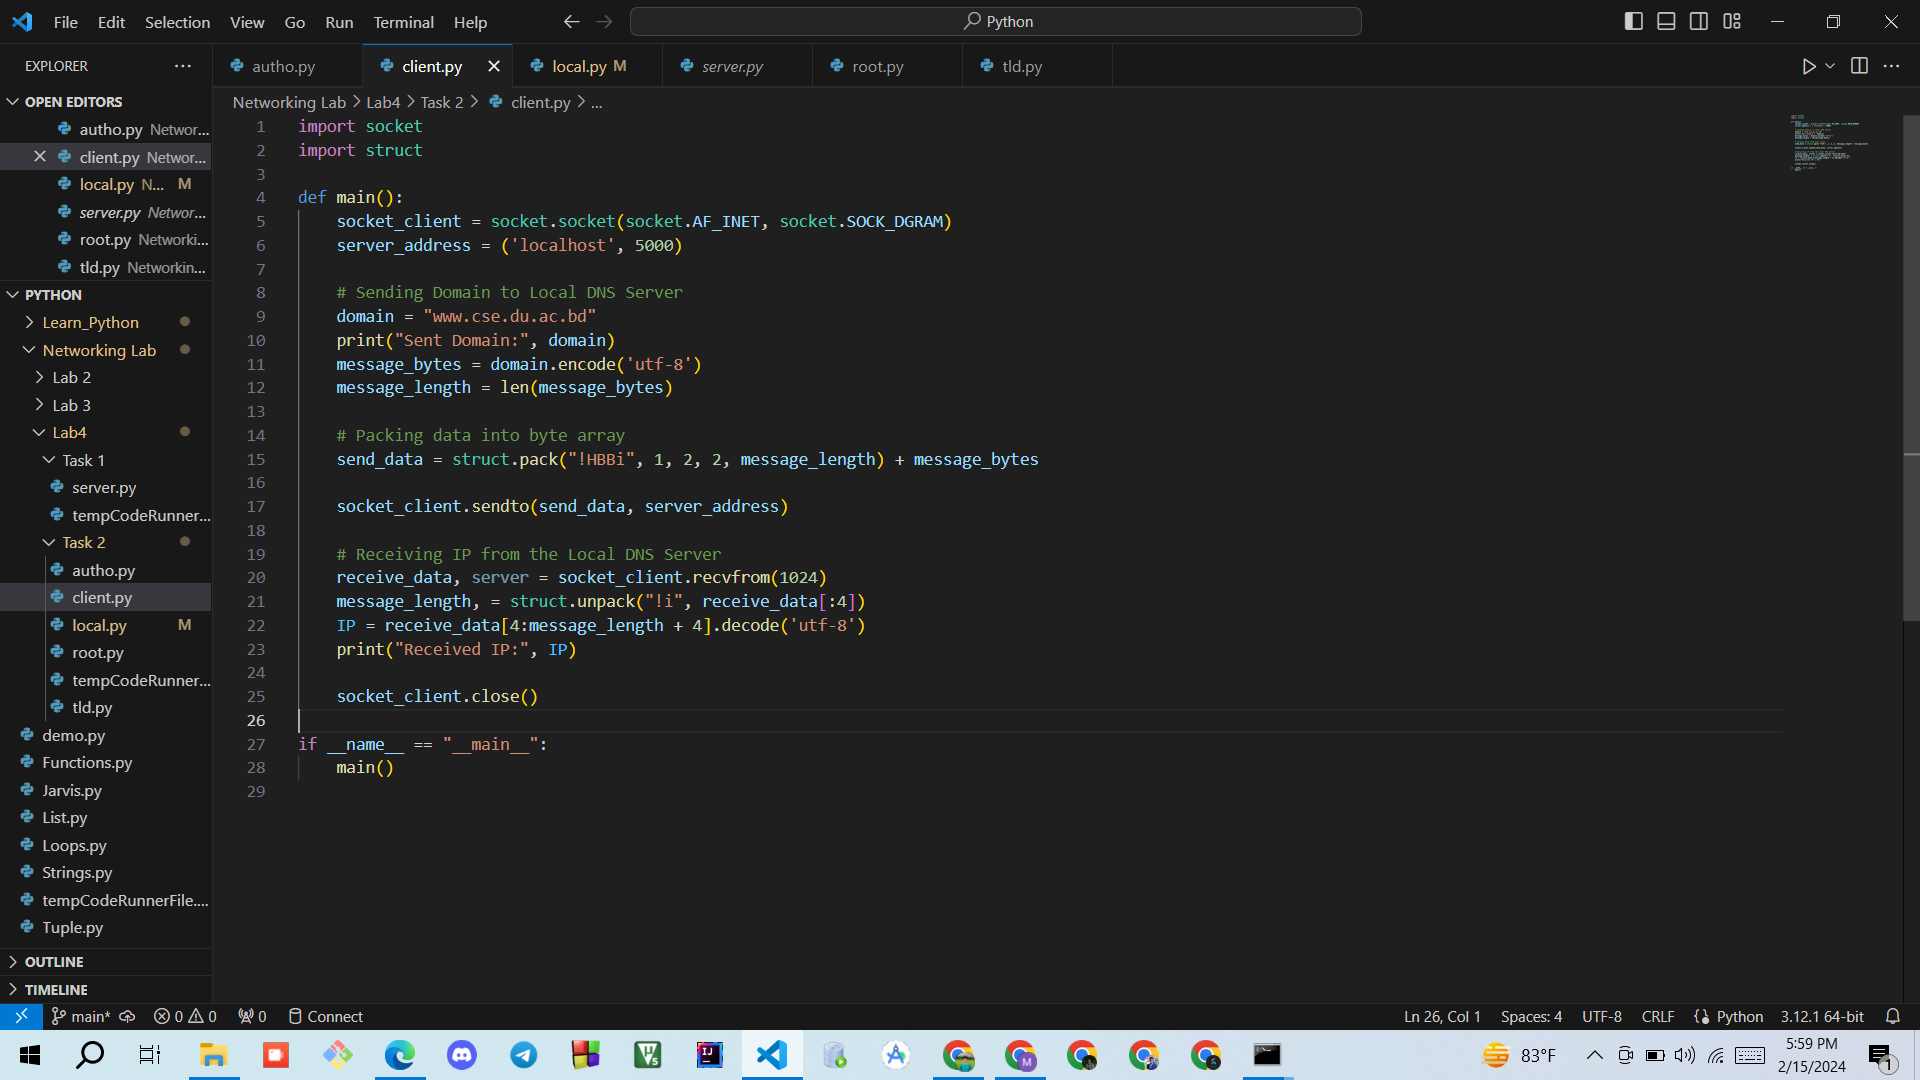
\includegraphics[width=0.8\textwidth]{Screenshot (164).png}
        \caption{Client side code}
        \label{fig:1}
    \end{figure}
    
    \begin{figure}[H]
        \centering
        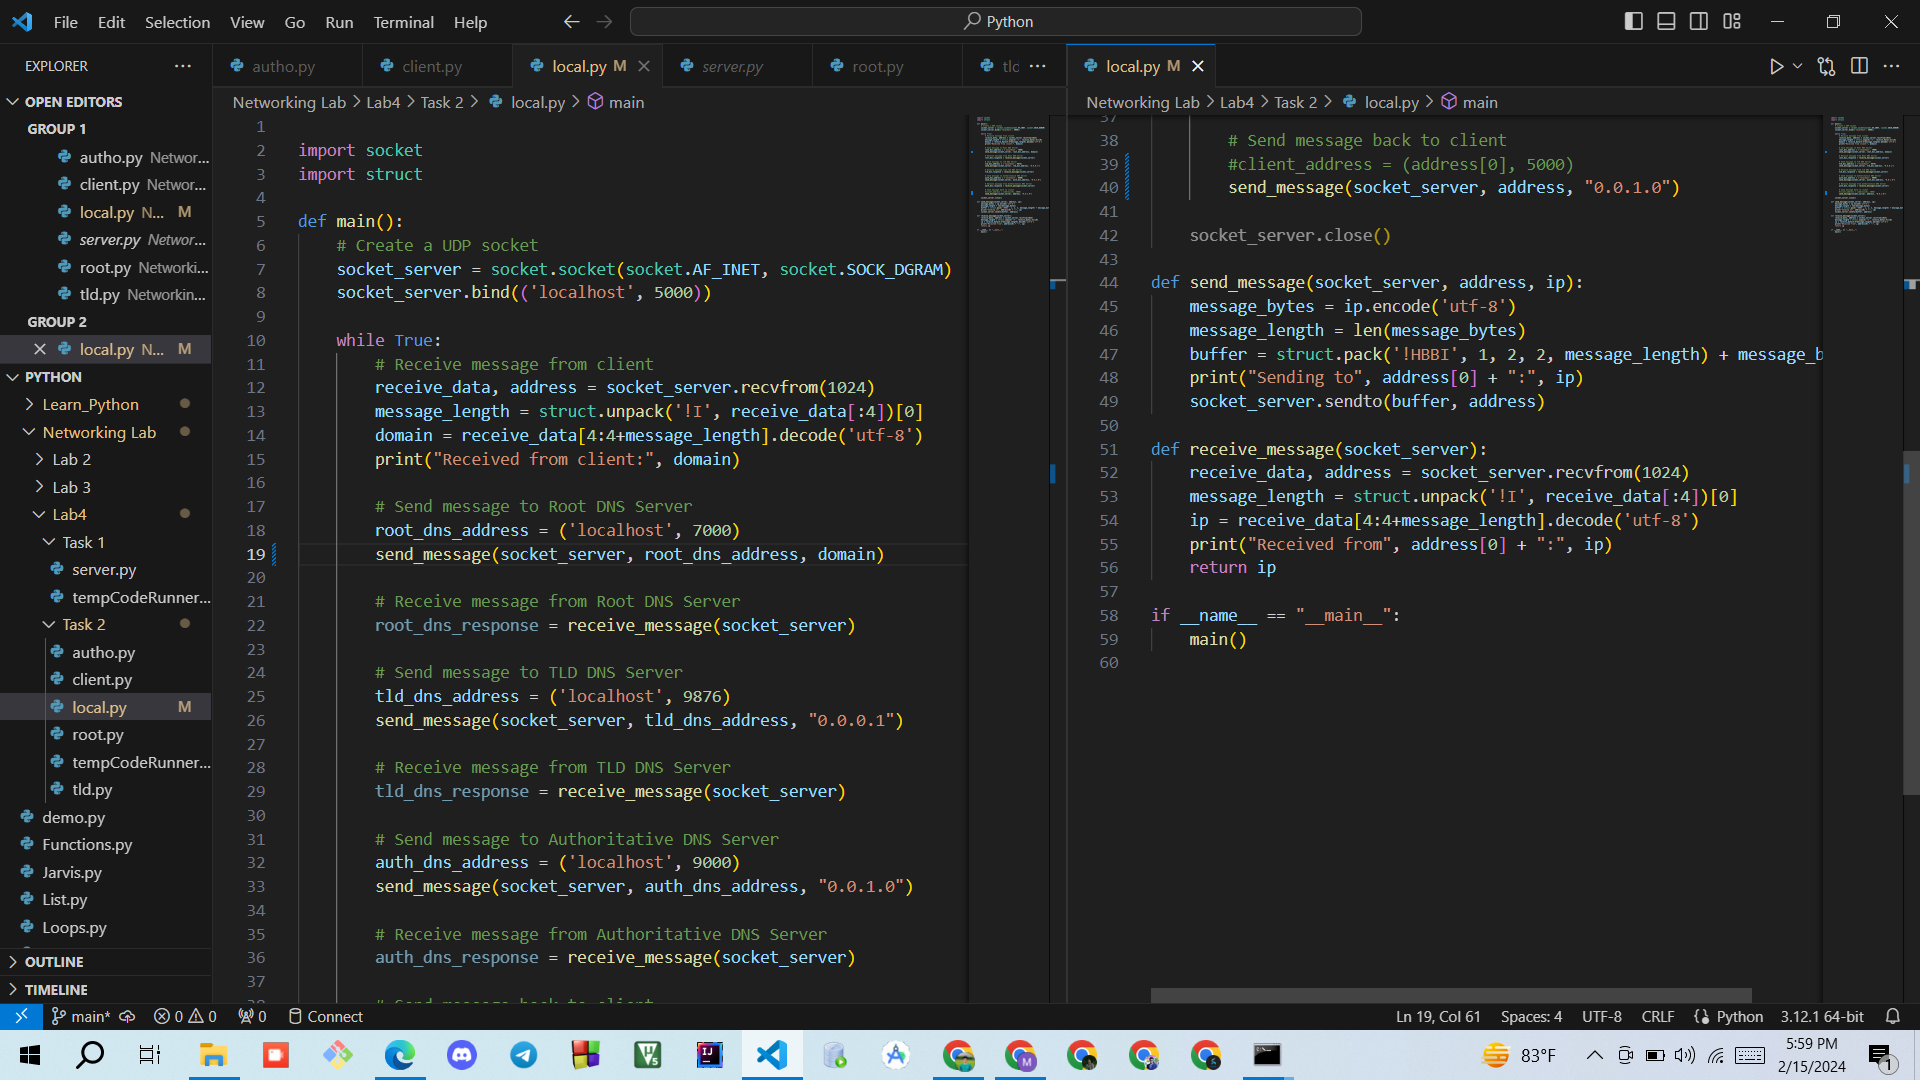
\includegraphics[width=0.8\textwidth]{Screenshot (165).png}
        \caption{Local Server Side Code}
        \label{fig:2}
    \end{figure}
    
    \begin{figure}[H]
      \centering
      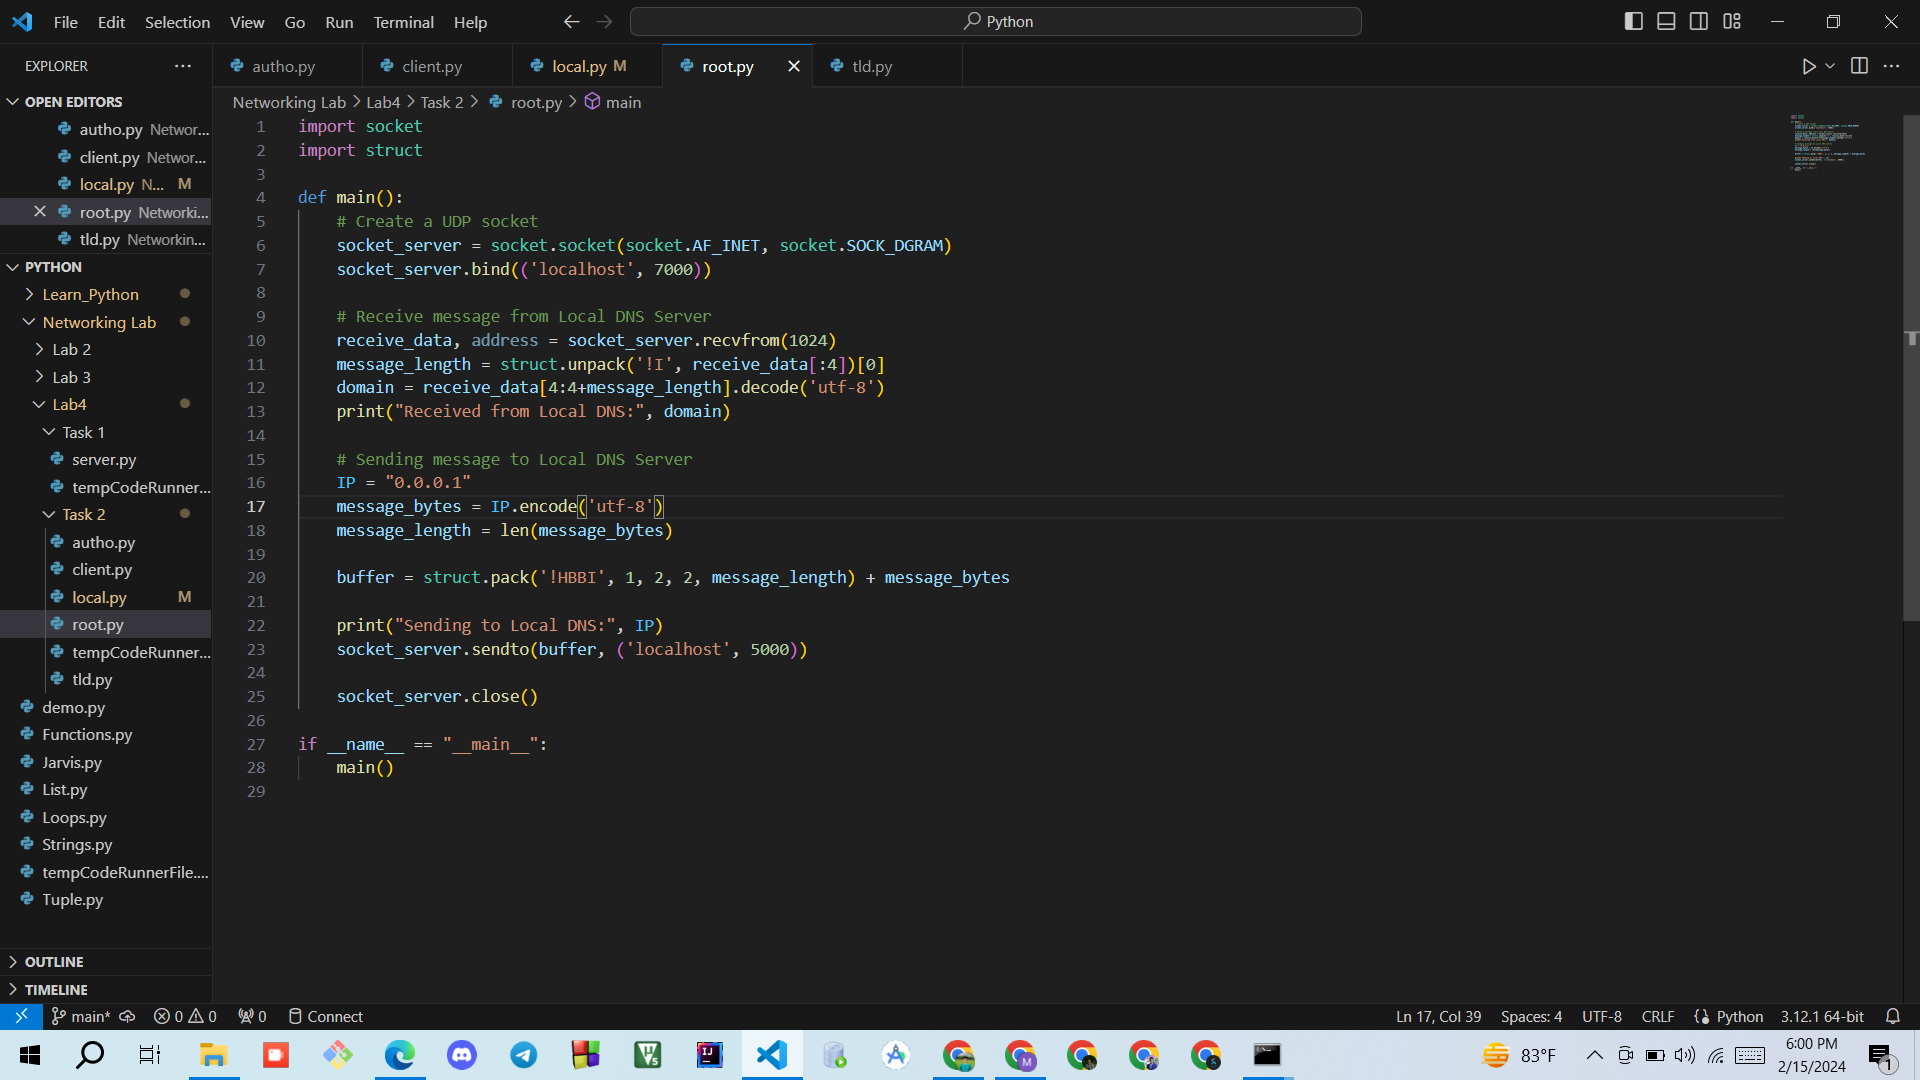
\includegraphics[width=0.8\textwidth]{Screenshot (166).png}
      \caption{Root Server Side Code}
      \label{fig:3}
    \end{figure}
    
    \begin{figure}[H]
      \centering
      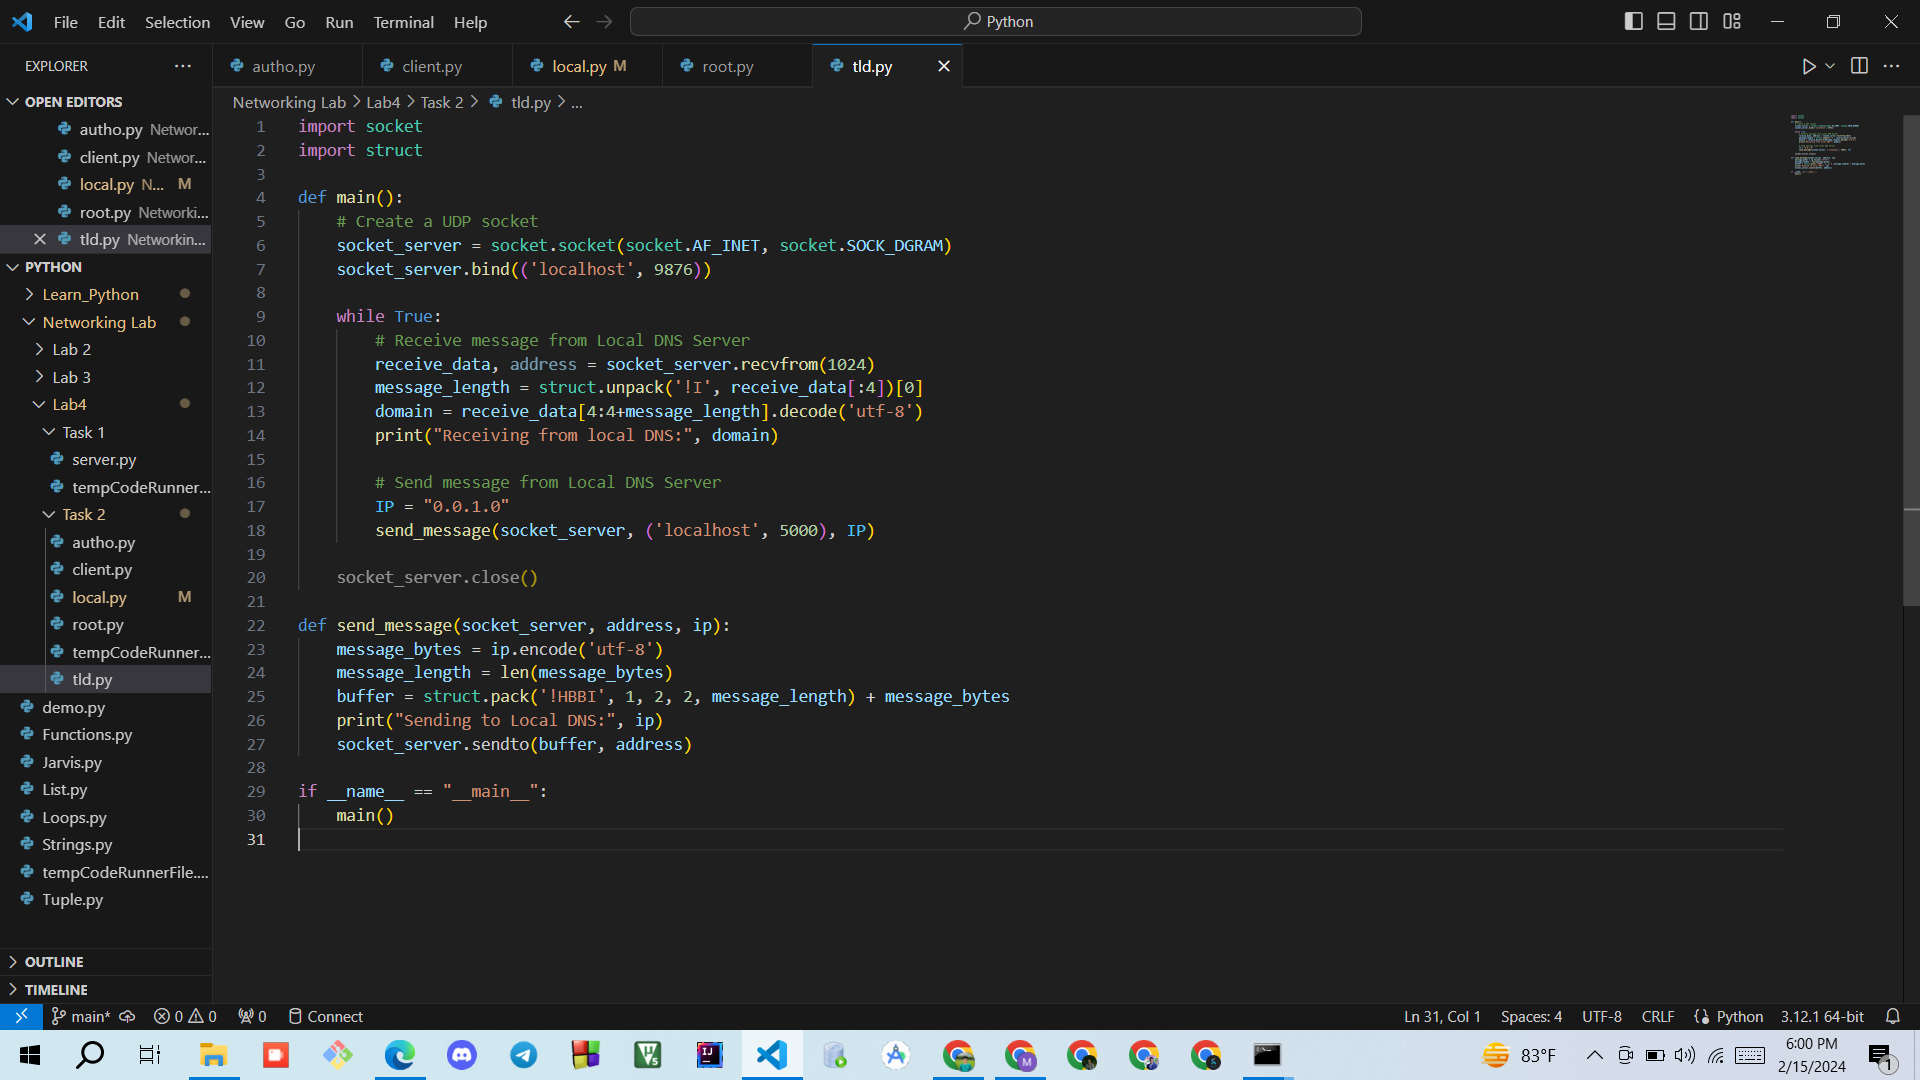
\includegraphics[width=0.8\textwidth]{Screenshot (167).png}
      \caption{TLD Server Side Code}
      \label{fig:4}
    \end{figure}


    \begin{figure}[H]
      \centering
      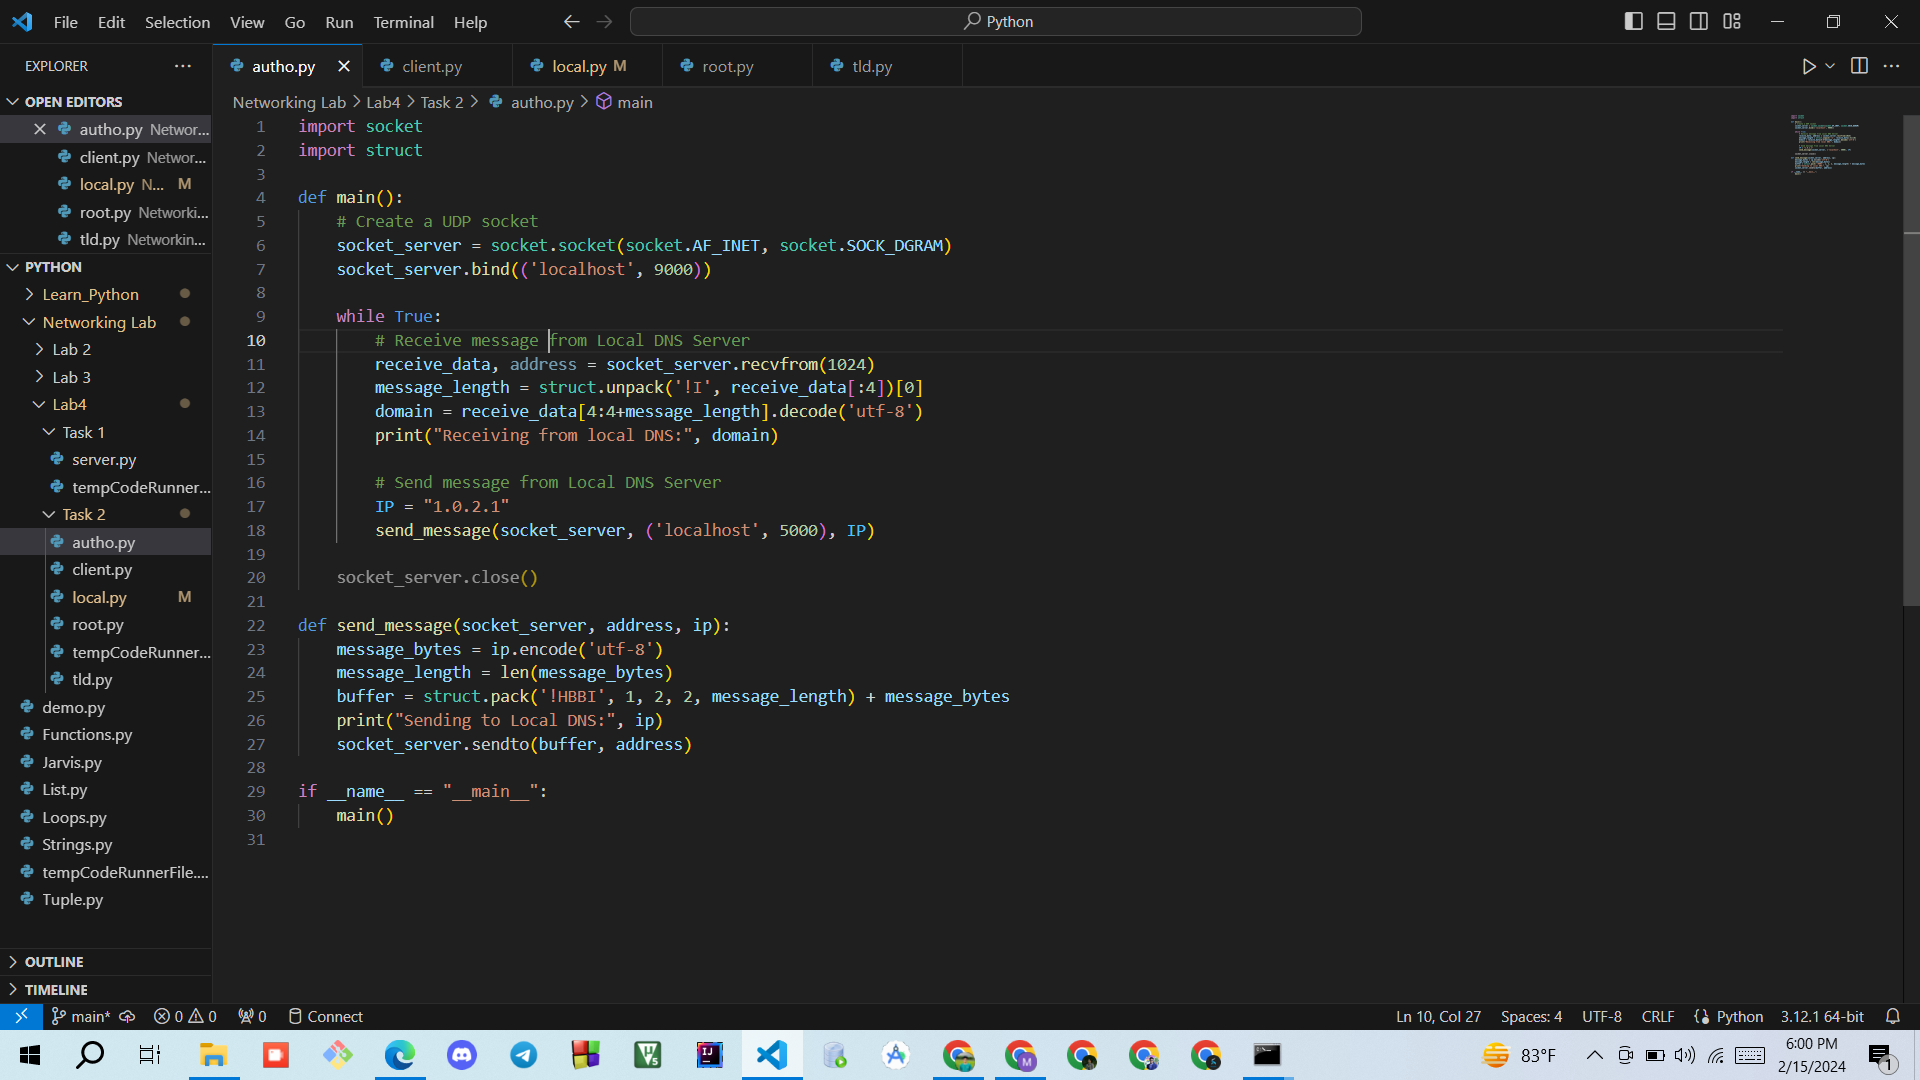
\includegraphics[width=0.8\textwidth]{Screenshot (168).png}
      \caption{Authorititive Server Side Code}
      \label{fig:4}
    \end{figure}



        \begin{figure}[H]
        \centering
        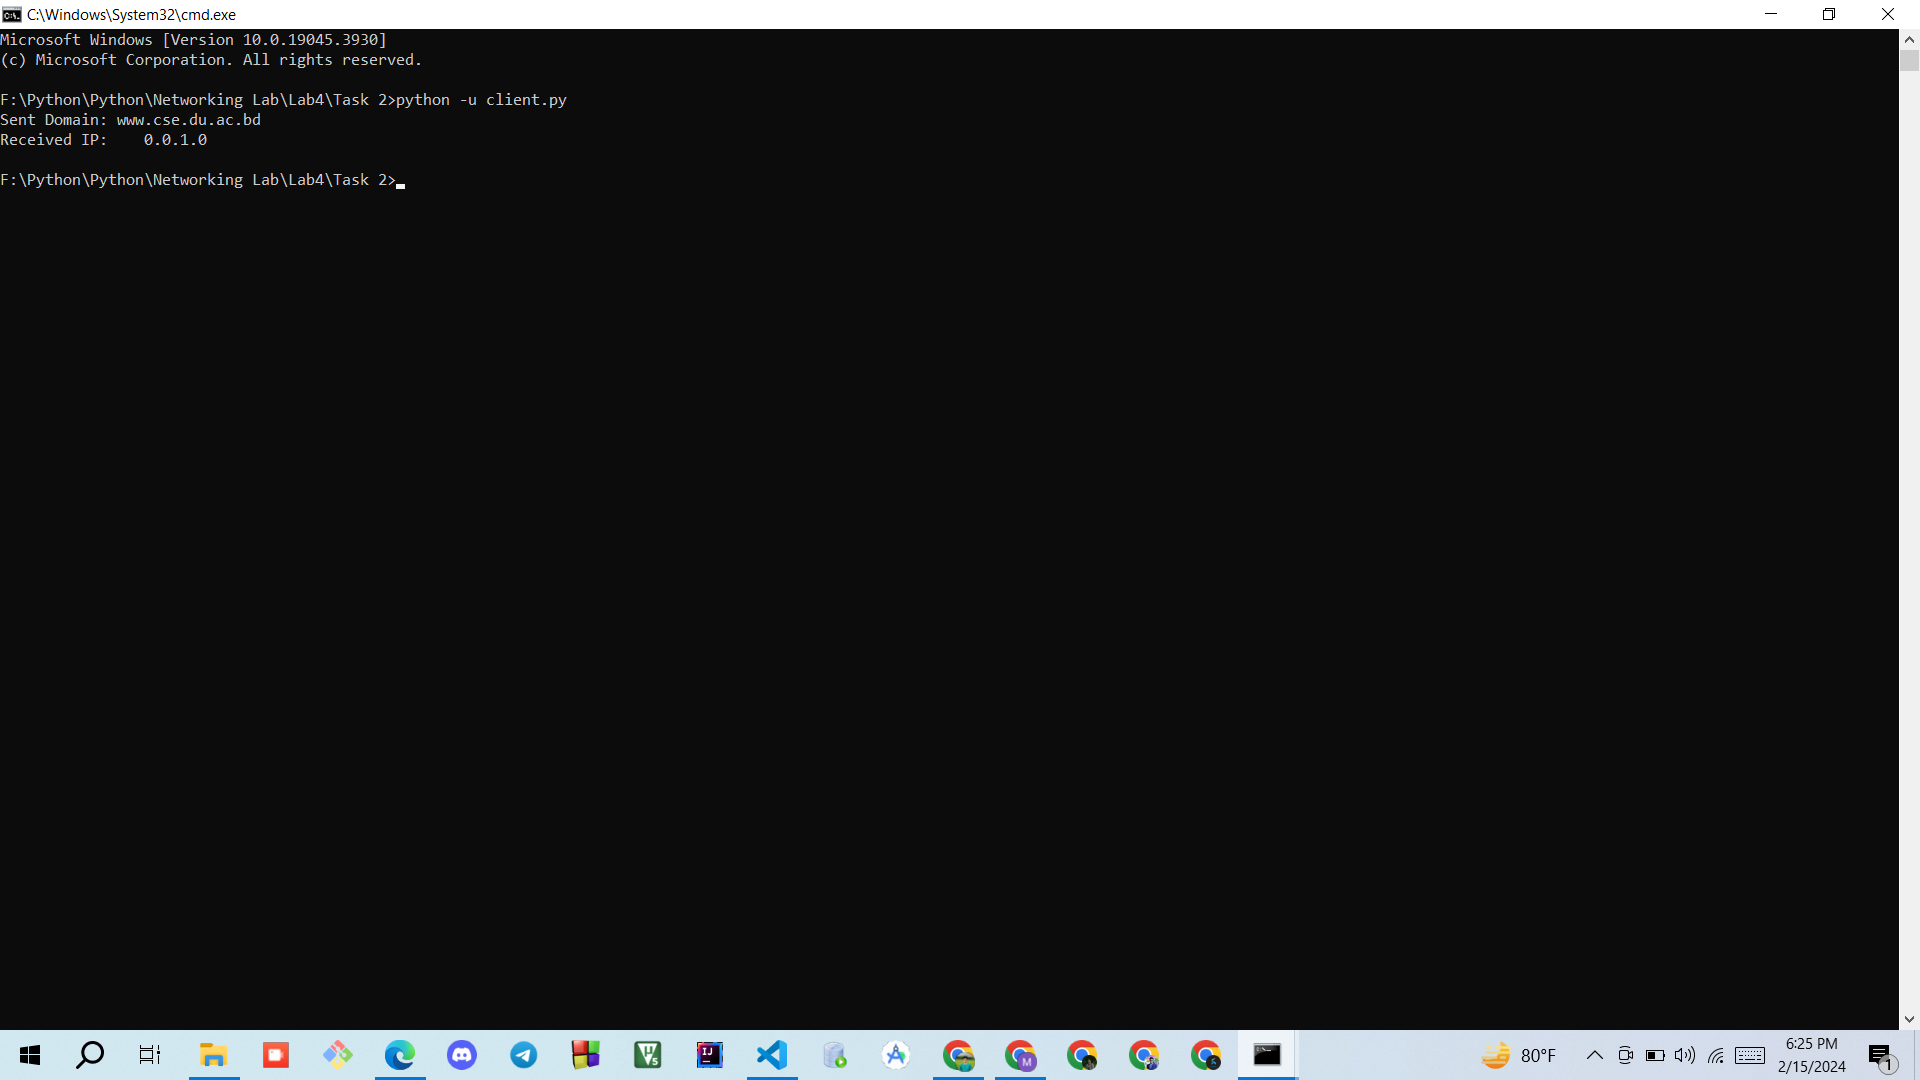
\includegraphics[width=0.8\textwidth]{Screenshot (169).png}
        \caption{Client Result side code}
        \label{fig:1}
    \end{figure}
    
    \begin{figure}[H]
        \centering
        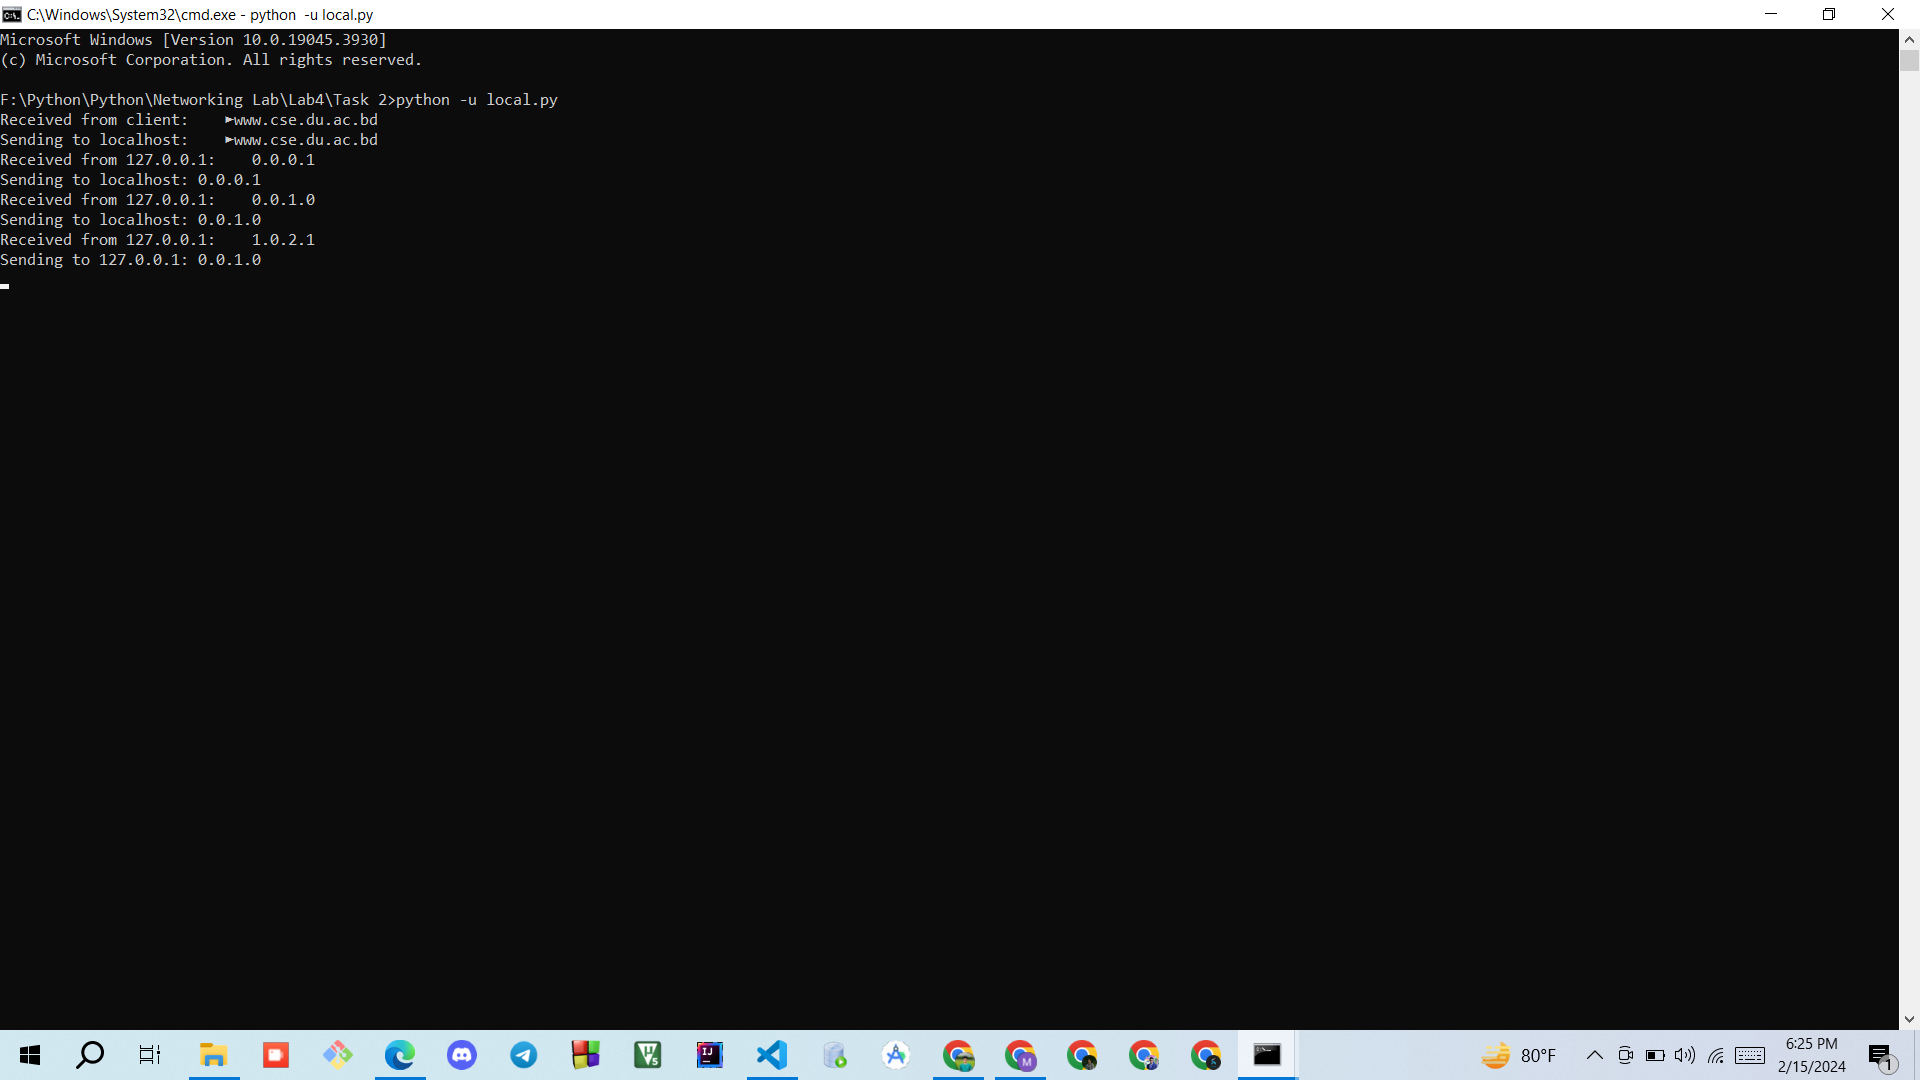
\includegraphics[width=0.8\textwidth]{Screenshot (170).png}
        \caption{Local Result Server Side Code}
        \label{fig:2}
    \end{figure}
    
    \begin{figure}[H]
      \centering
      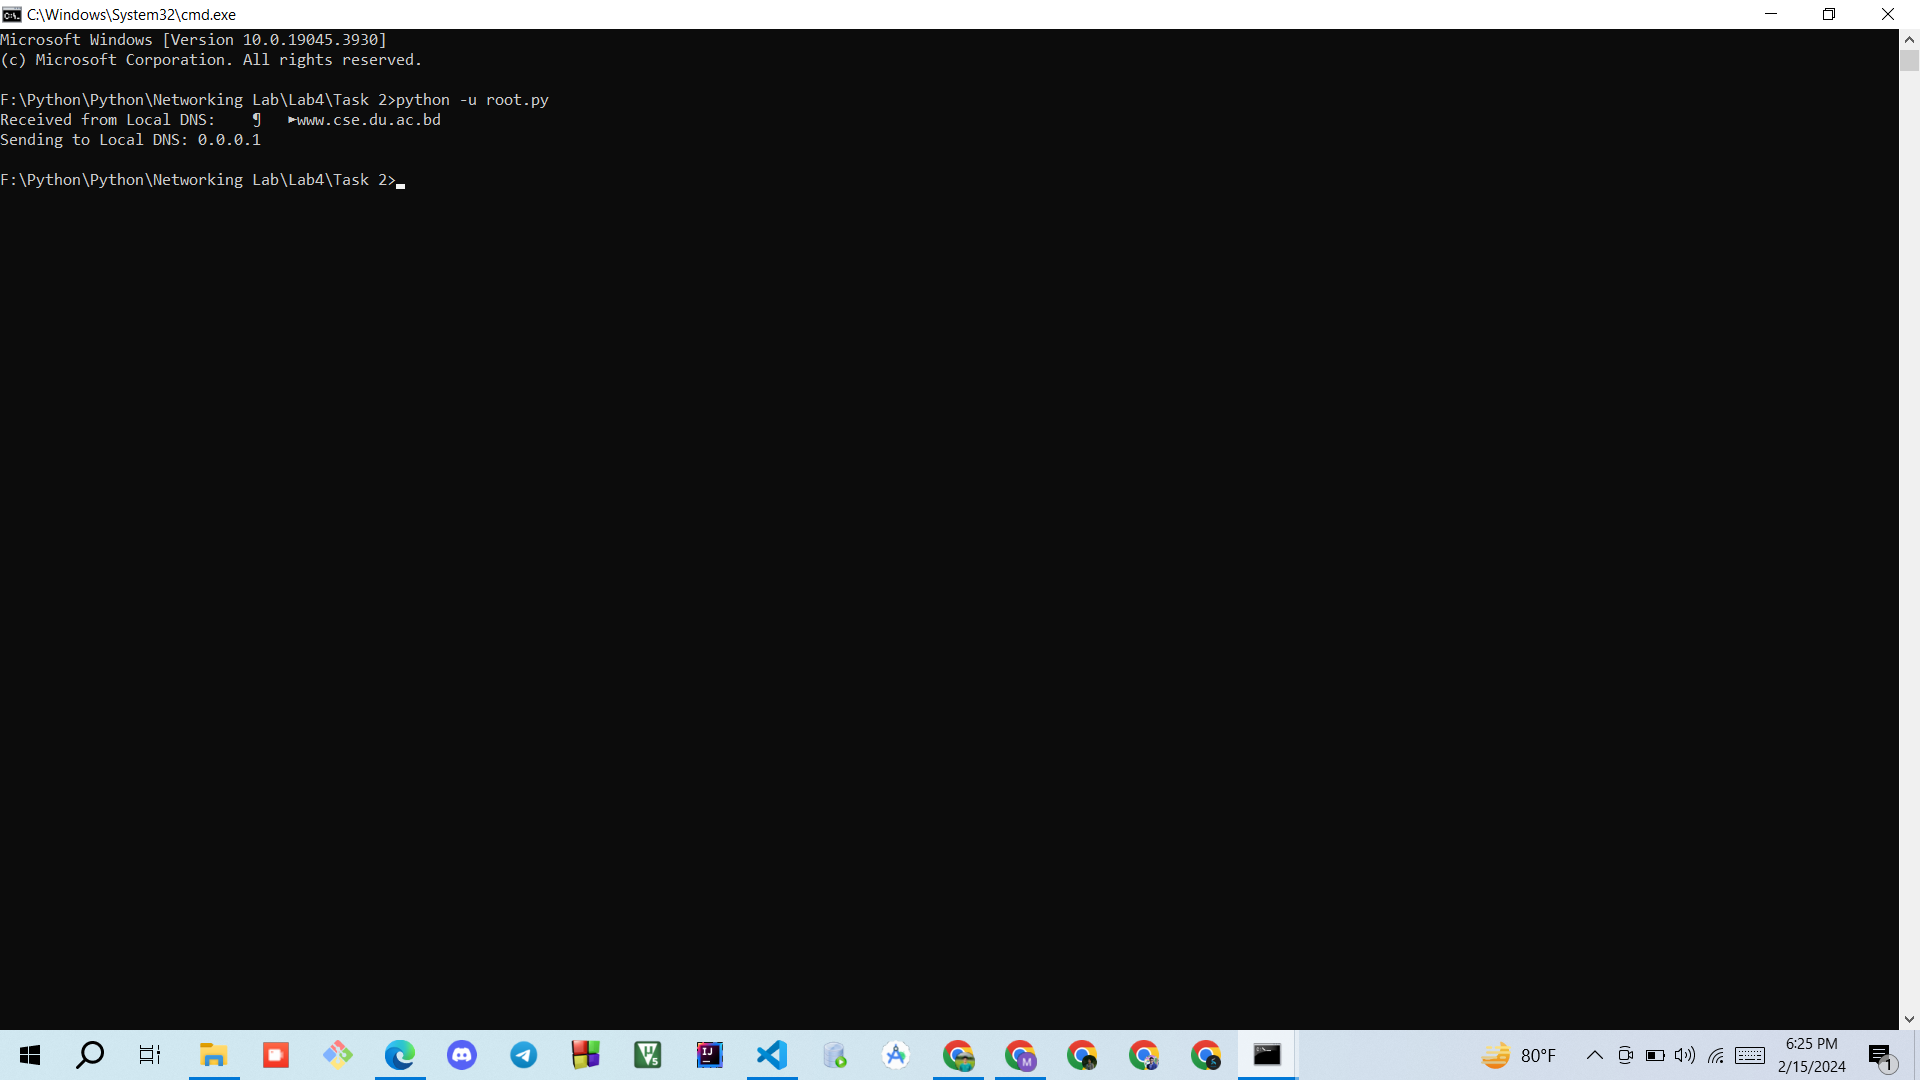
\includegraphics[width=0.8\textwidth]{Screenshot (171).png}
      \caption{Root Result Server Side Code}
      \label{fig:3}
    \end{figure}
    
    \begin{figure}[H]
      \centering
      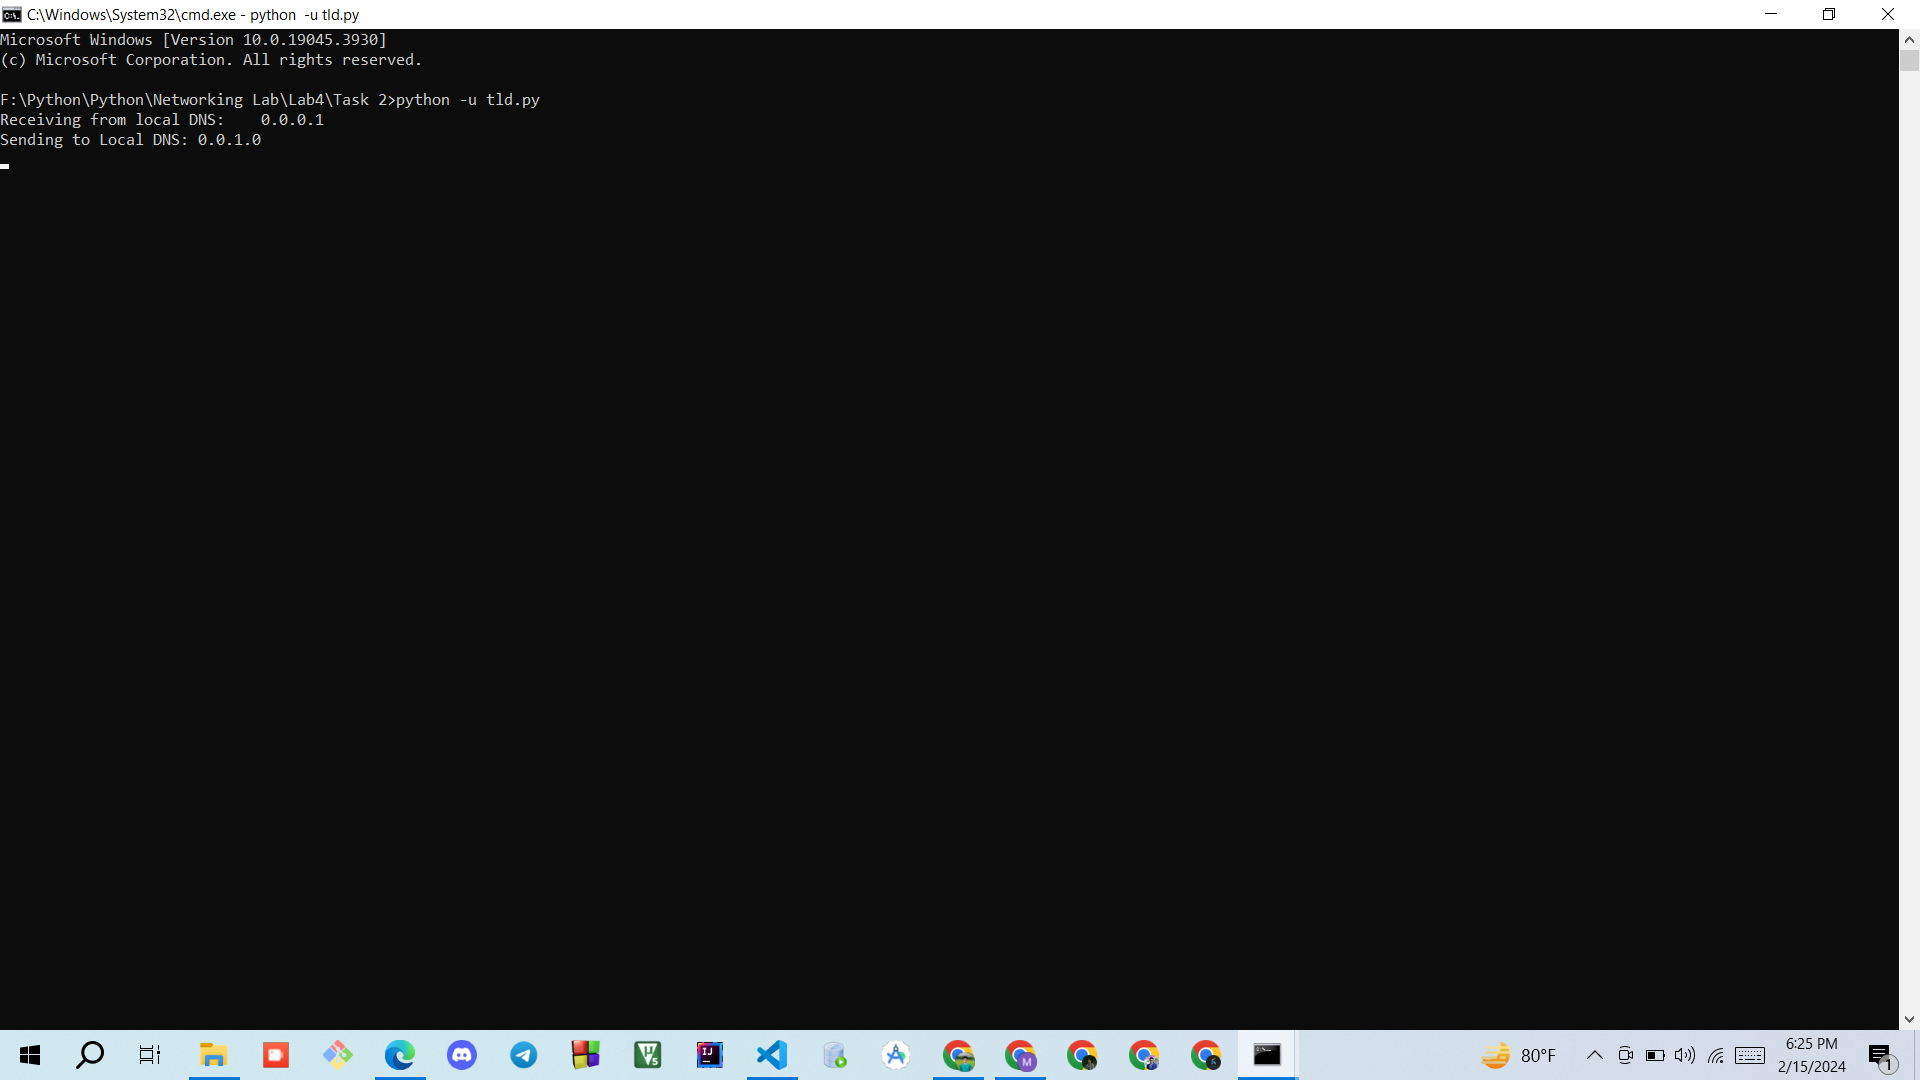
\includegraphics[width=0.8\textwidth]{Screenshot (172).png}
      \caption{TLD Result Server Side Code}
      \label{fig:4}
    \end{figure}


    \begin{figure}[H]
      \centering
      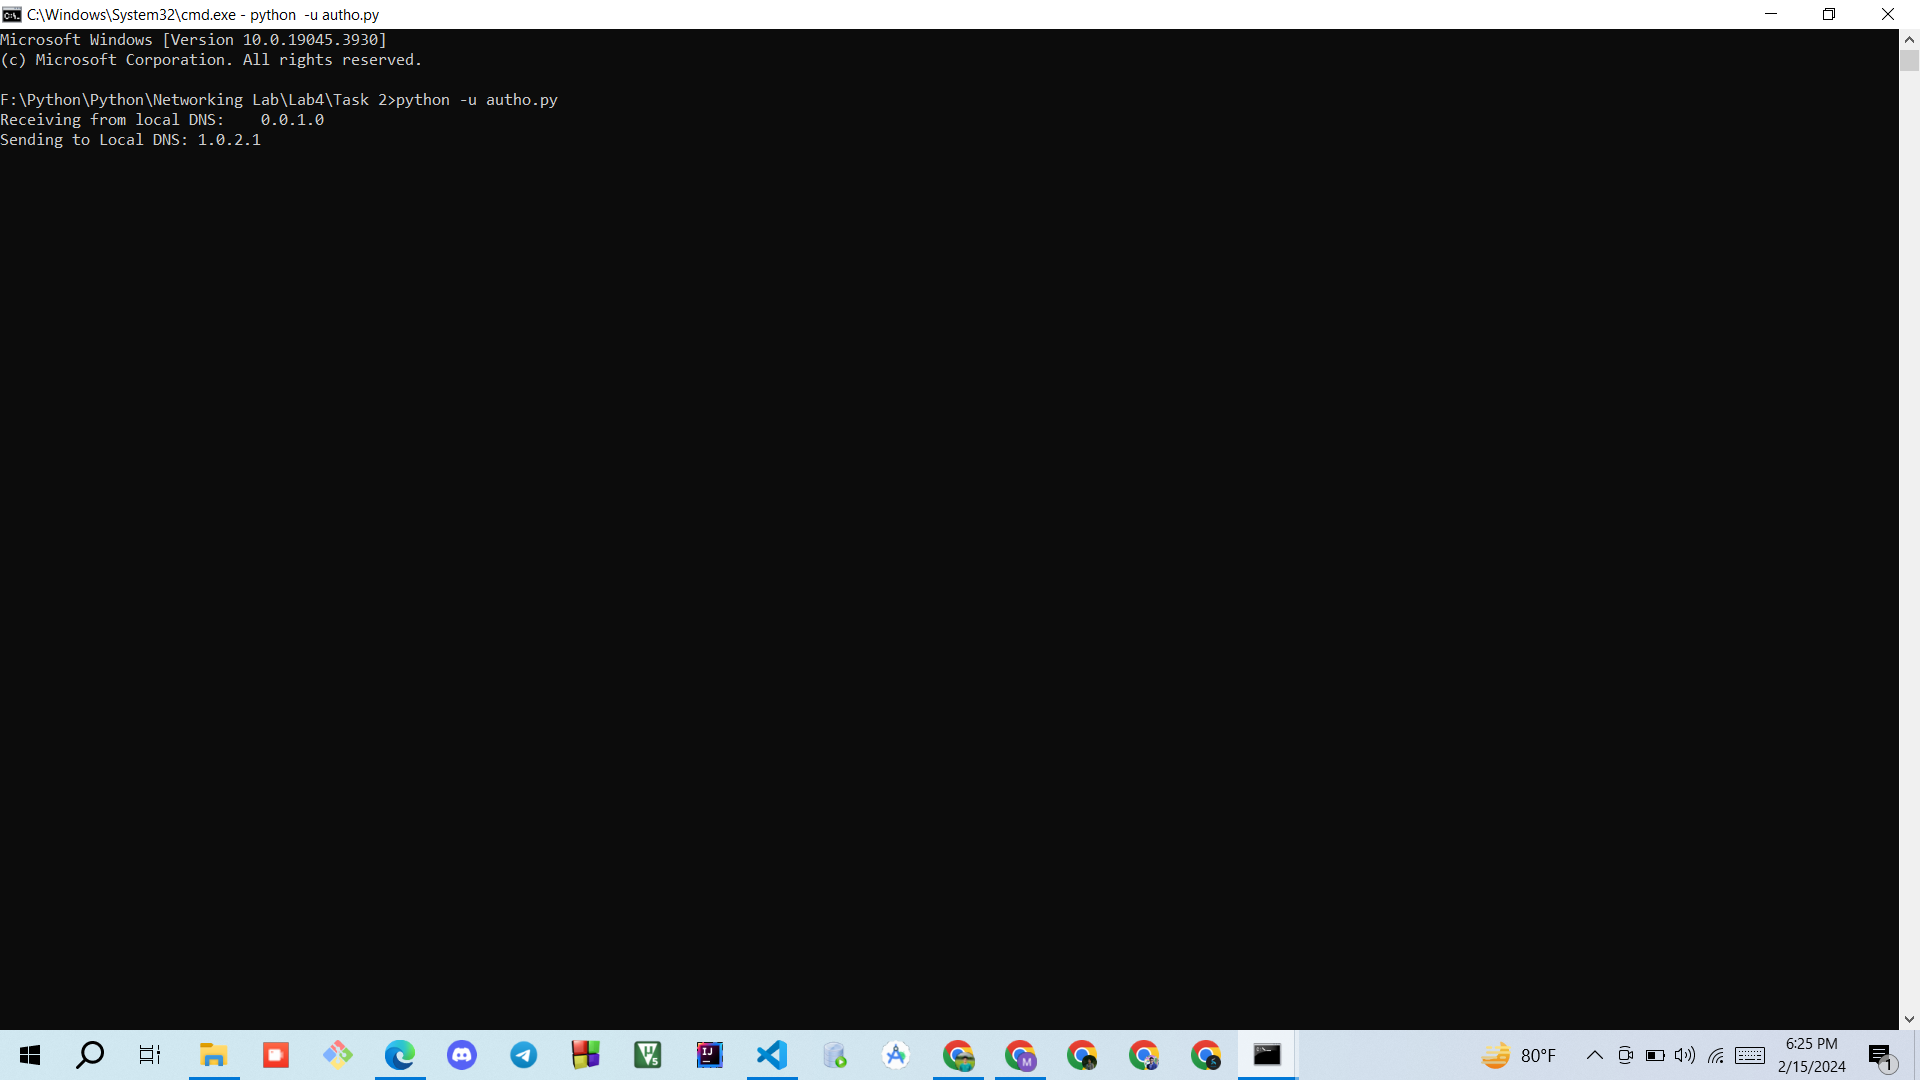
\includegraphics[width=0.8\textwidth]{Screenshot (173).png}
      \caption{Authorititive Result Server Side Code}
      \label{fig:4}
    \end{figure}

\end{itemize}

\subsection{Task 3}

\begin{itemize}
    \item \textbf{Recursive DNS resolution}
    
    
    \begin{minted}[mathescape, linenos]{python}
    Local DNS SERVER SIDE CODE
   
import socket
import struct

def main():
    server_socket = socket.socket(socket.AF_INET, socket.SOCK_DGRAM)
    server_socket.bind(('localhost', 5000))

    # Receive message from client
    receive_data, client_address = server_socket.recvfrom(1024)
    received_buffer = memoryview(receive_data)

    message_length = struct.unpack('!I', received_buffer[:4])[0]
    domain = received_buffer[4:4+message_length].tobytes().decode('utf-8')
    print("Received from client:", domain)

    # Send message to Root DNS Server
    root_dns_address = ('localhost', 7000)
    root_ip = "0.0.0.0"
    
    print("Sending to Root DNS:", root_ip)

    message_bytes2 = root_ip.encode('utf-8')
    message_length2 = len(message_bytes2)

    send_data = struct.pack('!HBBI', 1, 2, 2, message_length2) + message_bytes2

    server_socket.sendto(send_data, root_dns_address)

    # Receive message from Root DNS Server
    receive_data2, _ = server_socket.recvfrom(1024)
    received_buffer2 = memoryview(receive_data2)

    message_length3 = struct.unpack('!I', received_buffer2[:4])[0]
    domain2 = received_buffer2[4:4+message_length3].tobytes().decode('utf-8')
    print("Received from Root DNS:", domain2)

    # Send message to client
    client_ip = "1.1.1.1"

    print("Sending to Client:", client_ip)

    message_bytes5 = client_ip.encode('utf-8')
    message_length5 = len(message_bytes5)

    send_data2 = struct.pack('!HBBI', 1, 2, 2, message_length5) + message_bytes5

    server_socket.sendto(send_data2, client_address)

if __name__ == "__main__":
    main()



\end{minted}

 \begin{minted}[mathescape, linenos]{python}
    Root DNS SERVER SIDE CODE
    import socket
import struct

def main():
    server_socket = socket.socket(socket.AF_INET, socket.SOCK_DGRAM)
    server_socket.bind(('localhost', 7000))

    # Receive message from Local DNS Server
    receive_data, local_dns_address = server_socket.recvfrom(1024)
    received_buffer = memoryview(receive_data)

    message_length = struct.unpack('!I', received_buffer[:4])[0]
    domain = received_buffer[4:4+message_length].tobytes().decode('utf-8')
    print("Received from Local DNS:", domain)

    # Send message to Root TLD DNS Server
    tld_dns_address = ('localhost', 9800)
    tld_ip = "0.0.1.0"

    print("Sending to TLD DNS:", tld_ip)

    message_bytes2 = tld_ip.encode('utf-8')
    message_length2 = len(message_bytes2)

    send_data = struct.pack('!HBBI', 1, 2, 2, message_length2) + message_bytes2

    server_socket.sendto(send_data, tld_dns_address)

    # Receive message from TLD DNS Server
    receive_data2, _ = server_socket.recvfrom(1024)
    received_buffer2 = memoryview(receive_data2)

    message_length3 = struct.unpack('!I', received_buffer2[:4])[0]
    domain2 = received_buffer2[4:4+message_length3].tobytes().decode('utf-8')
    print("Received from TLD DNS:", domain2)

    # Send message to Local DNS Server
    local_dns_ip = "1.1.1.1"

    print("Sending to Local DNS:", local_dns_ip)

    message_bytes5 = local_dns_ip.encode('utf-8')
    message_length5 = len(message_bytes5)

    send_data2 = struct.pack('!HBBI', 1, 2, 2, message_length5) + message_bytes5

    server_socket.sendto(send_data2, local_dns_address)

if __name__ == "__main__":
    main()

   
\end{minted}
 \begin{minted}[mathescape, linenos]{python}
    TLD DNS SERVER SIDE CODE
   import socket
import struct

def main():
    server_socket = socket.socket(socket.AF_INET, socket.SOCK_DGRAM)
    server_socket.bind(('localhost', 9800))

    # Receive message from Root DNS Server
    receive_data, root_dns_address = server_socket.recvfrom(1024)
    received_buffer = memoryview(receive_data)

    message_length = struct.unpack('!I', received_buffer[:4])[0]
    domain = received_buffer[4:4+message_length].tobytes().decode('utf-8')
    print("Received from Root DNS:", domain)

    # Send message to Auth DNS Server
    auth_dns_address = ('localhost', 9000)
    auth_ip = "1.1.0.0"

    print("Sending to Auth DNS:", auth_ip)

    message_bytes2 = auth_ip.encode('utf-8')
    message_length2 = len(message_bytes2)

    send_data = struct.pack('!HBBI', 1, 2, 2, message_length2) + message_bytes2

    server_socket.sendto(send_data, auth_dns_address)

    # Receive message from Auth DNS Server
    receive_data2, _ = server_socket.recvfrom(1024)
    received_buffer2 = memoryview(receive_data2)

    message_length3 = struct.unpack('!I', received_buffer2[:4])[0]
    domain2 = received_buffer2[4:4+message_length3].tobytes().decode('utf-8')
    print("Received from Auth DNS:", domain2)

    # Send message to Root DNS Server
    root_dns_ip = "1.1.1.1"

    print("Sending to Root DNS:", root_dns_ip)

    message_bytes5 = root_dns_ip.encode('utf-8')
    message_length5 = len(message_bytes5)

    send_data2 = struct.pack('!HBBI', 1, 2, 2, message_length5) + message_bytes5

    server_socket.sendto(send_data2, root_dns_address)

if __name__ == "__main__":
    main()

\end{minted}
 \begin{minted}[mathescape, linenos]{python}
    Authoritative DNS SERVER SIDE CODE
    import socket
import struct

def main():
    # Receiving message from TLD DNS Server
    server_socket = socket.socket(socket.AF_INET, socket.SOCK_DGRAM)
    server_socket.bind(('localhost', 9000))

    receive_data, address = server_socket.recvfrom(1024)
    received_buffer = memoryview(receive_data)

    message_length = struct.unpack('!I', received_buffer[:4])[0]
    domain = received_buffer[4:4+message_length].tobytes().decode('utf-8')
    print("Received from TLD DNS:", domain)

    # Sending message to TLD DNS Server
    client_socket = socket.socket(socket.AF_INET, socket.SOCK_DGRAM)

    ip = "1.1.1.1"
    message_bytes2 = ip.encode('utf-8')
    message_length2 = len(message_bytes2)

    print("Sending to TLD DNS:", ip)

    send_data = struct.pack('!HBBI', 1, 2, 2, message_length2) + message_bytes2

    client_socket.sendto(send_data, ('localhost', 9800))

    server_socket.close()
    client_socket.close()

if __name__ == "__main__":
    main()

   
\end{minted}
 \begin{minted}[mathescape, linenos]{python}
    Client SIDE CODE
  import socket
import struct

def main():
    client_socket = socket.socket(socket.AF_INET, socket.SOCK_DGRAM)
    server_address = ('localhost', 5000)

    # Sending Domain to Local DNS Server
    domain = "www.cse.du.ac.bd"
    print("Sending domain:", domain)
    message_bytes = domain.encode('utf-8')
    message_length = len(message_bytes)

    send_data = struct.pack('!HBBI', 1, 2, 2, message_length) + message_bytes

    client_socket.sendto(send_data, server_address)

    # Receiving IP from the Local DNS Server
    receive_data, _ = client_socket.recvfrom(1024)
    received_buffer = memoryview(receive_data)

    query_id2, query_type2, query_class2, message_length2 = struct.unpack('!HBBI', received_buffer[:8])
    message_bytes2 = received_buffer[8:8+message_length2].tobytes()
    received_ip = message_bytes2.decode('utf-8')

    print("Received IP:", received_ip)

    client_socket.close()

if __name__ == "__main__":
    main()


\end{minted}


    \begin{figure}[H]
        \centering
        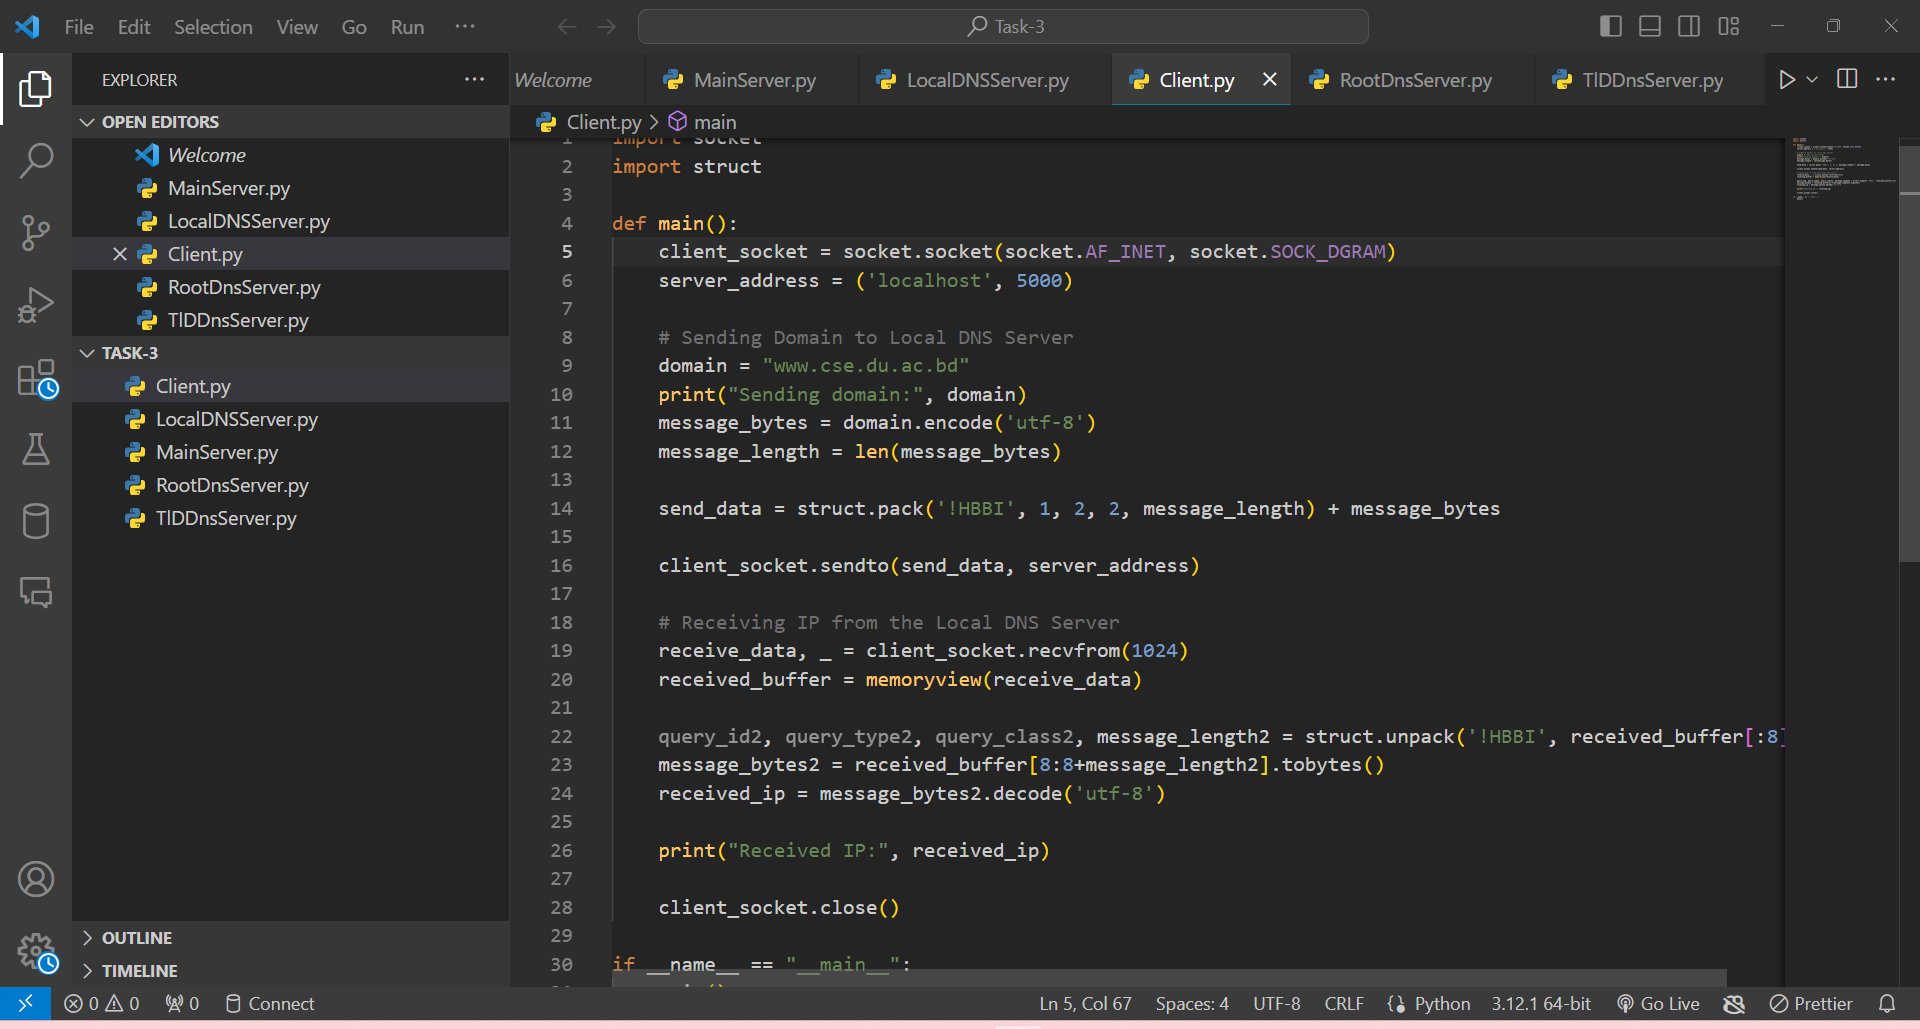
\includegraphics[width=0.8\textwidth]{client.png}
        \caption{Client side code}
        \label{fig:1}
    \end{figure}
    
    \begin{figure}[H]
        \centering
        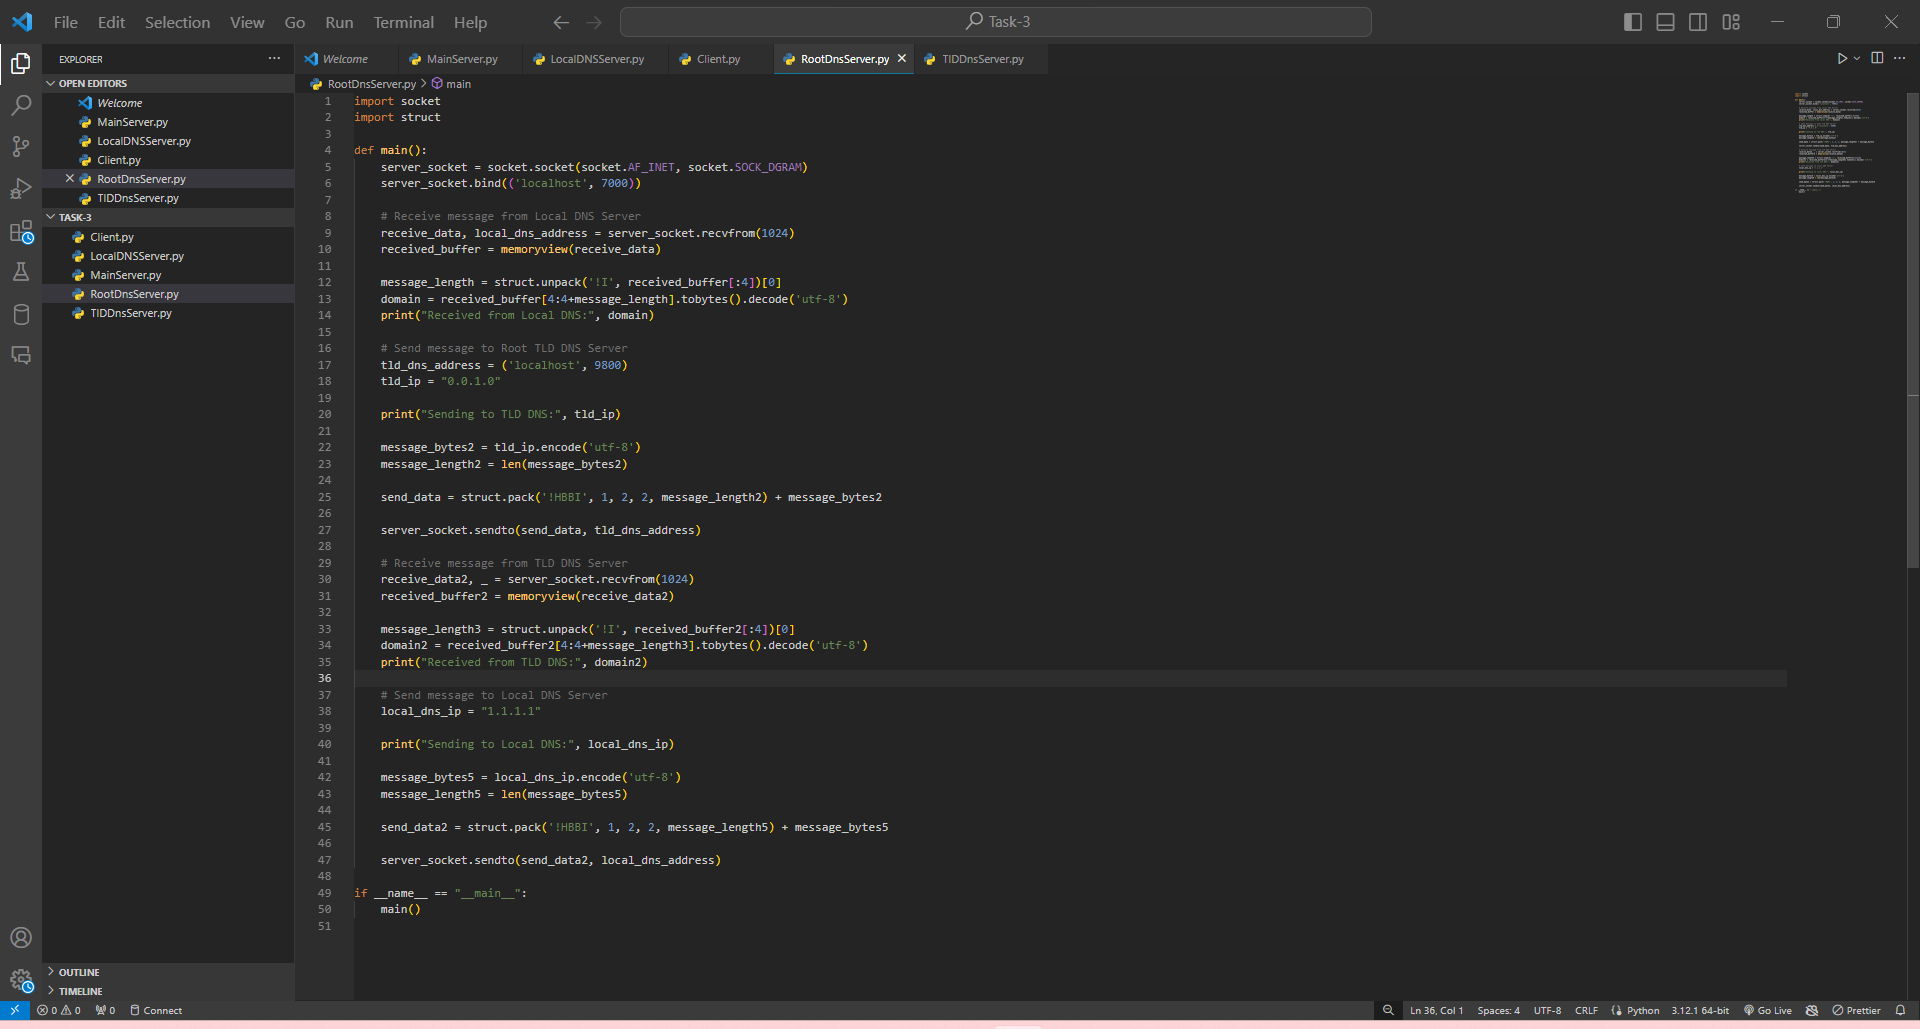
\includegraphics[width=0.8\textwidth]{RootDNSServer.png}
        \caption{Root DNS Server Side Code}
        \label{fig:2}
    \end{figure}
    \begin{figure}[H]
        \centering
        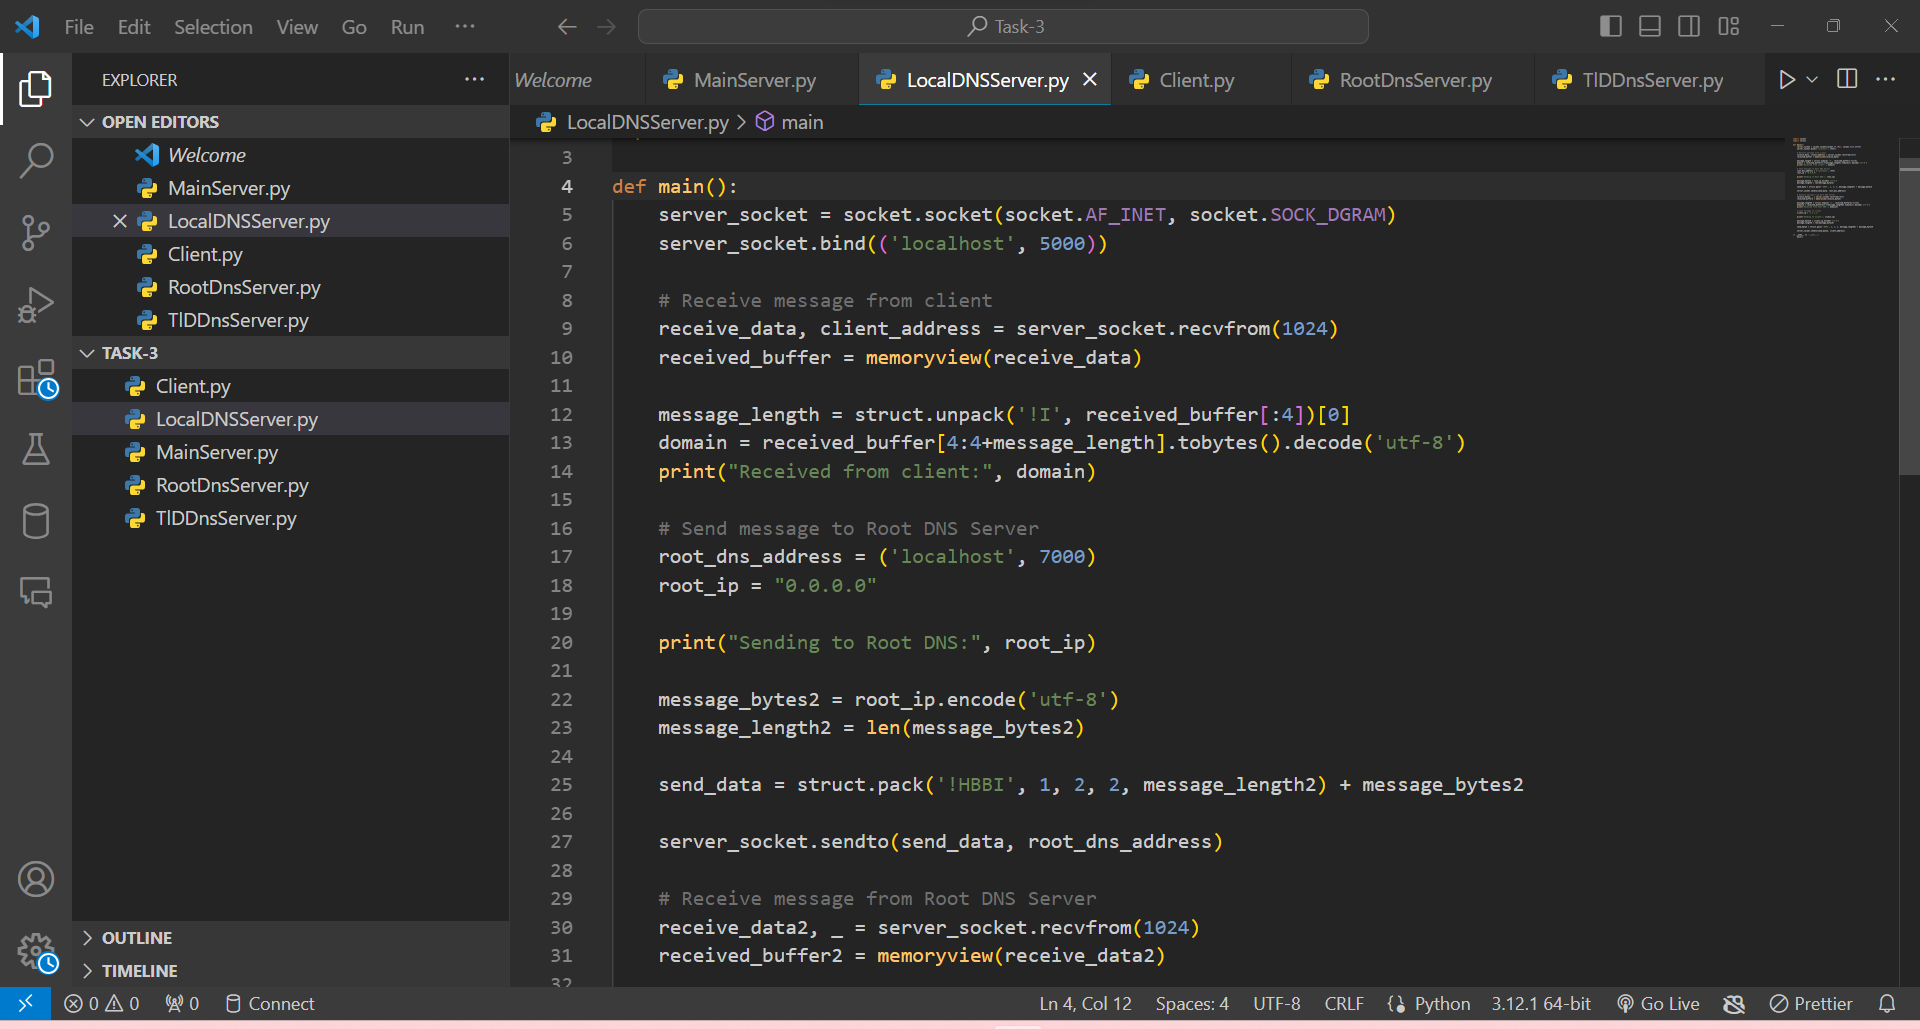
\includegraphics[width=0.8\textwidth]{LocalDNSServer.png}
        \caption{Local DNS Server Side Code}
        \label{fig:2}
    \end{figure}
    \begin{figure}[H]
        \centering
        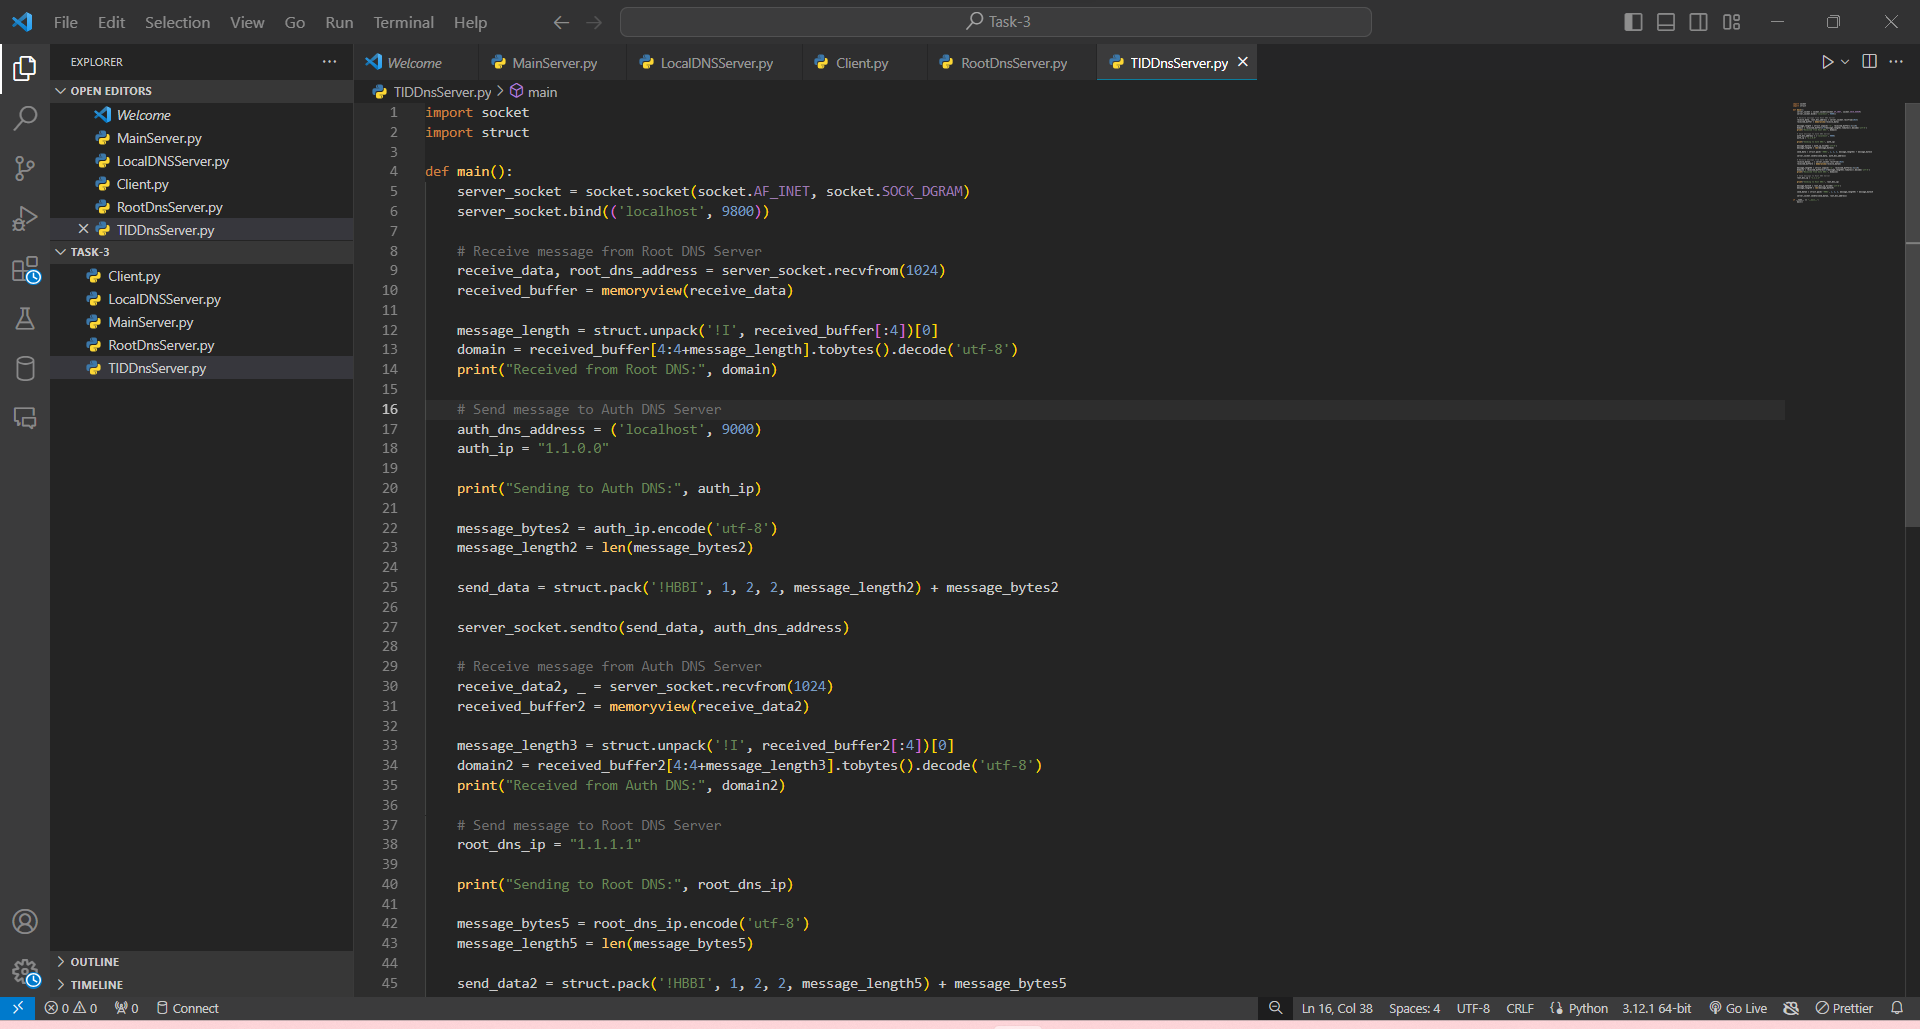
\includegraphics[width=0.8\textwidth]{TlDDNSServer.png}
        \caption{TLD DNS Server Side Code}
        \label{fig:2}
    \end{figure}
    \begin{figure}[H]
        \centering
        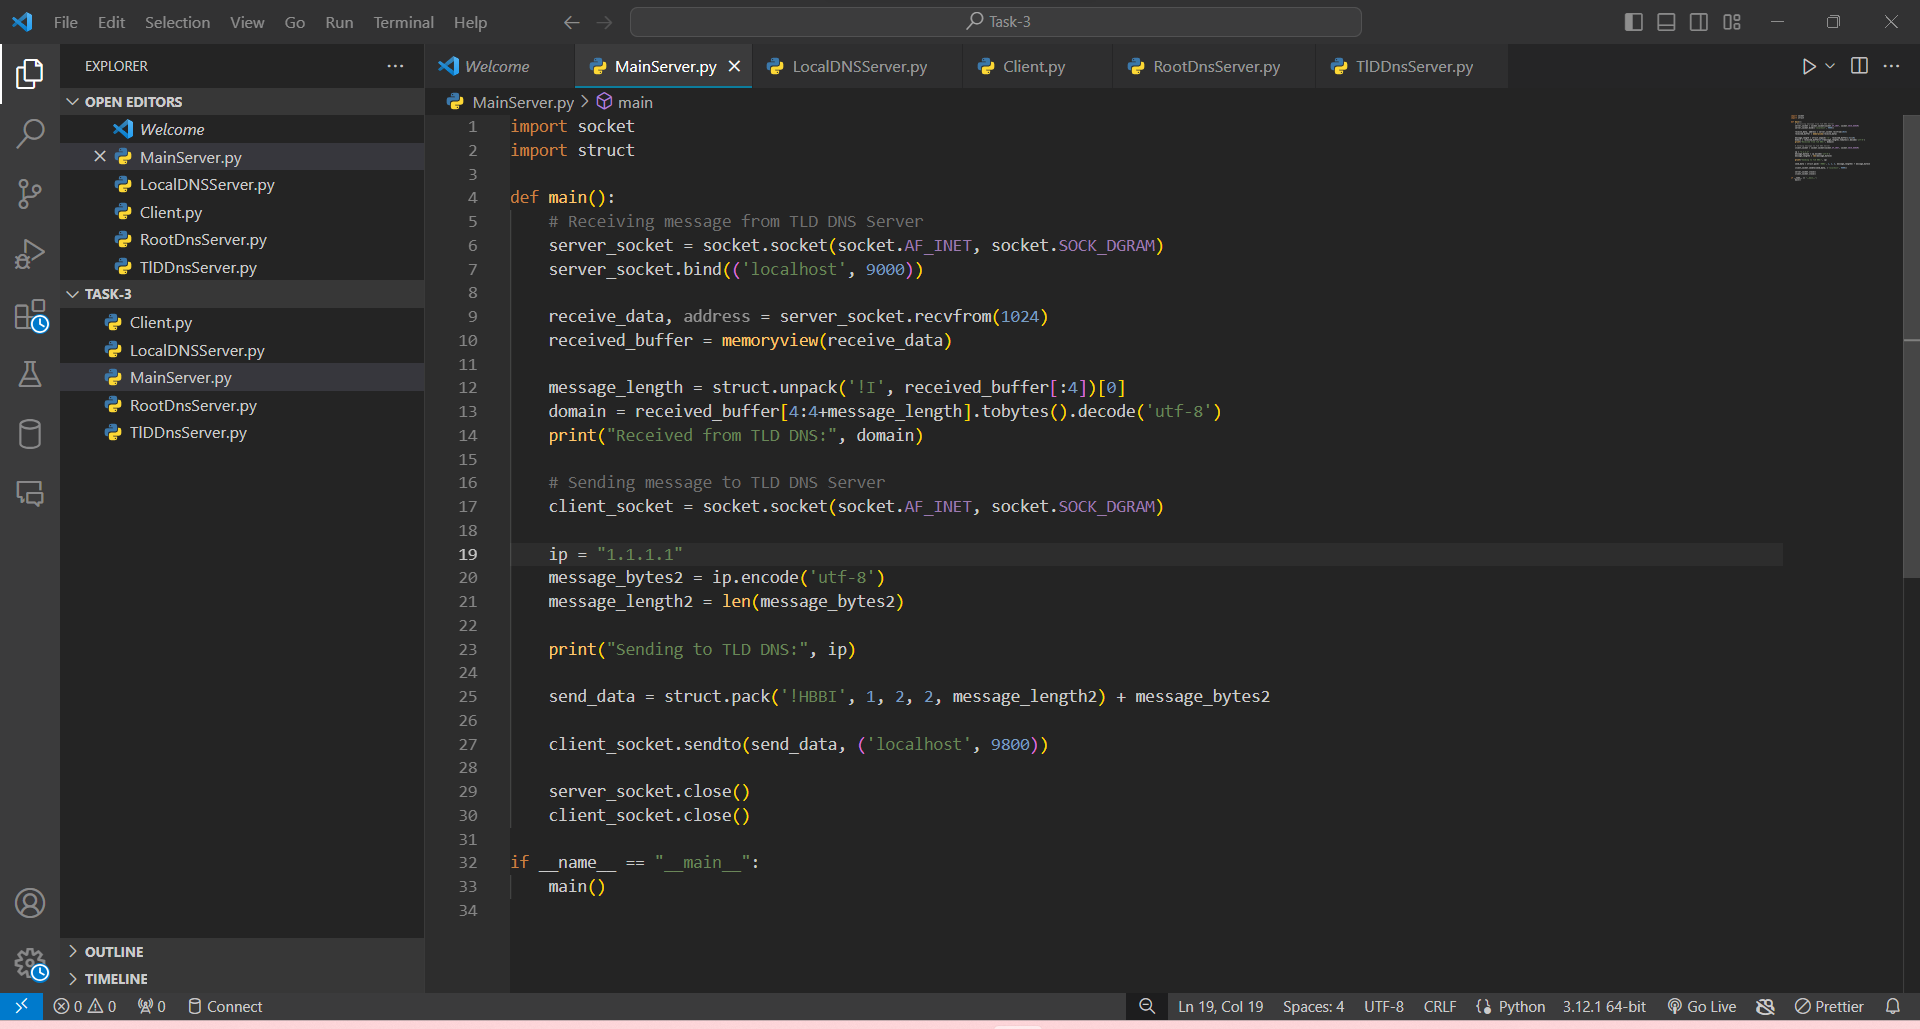
\includegraphics[width=0.8\textwidth]{MainServer.png}
        \caption{Authoritative Server Side Code}
        \label{fig:2}
    \end{figure}
     \begin{figure}[H]
        \centering
        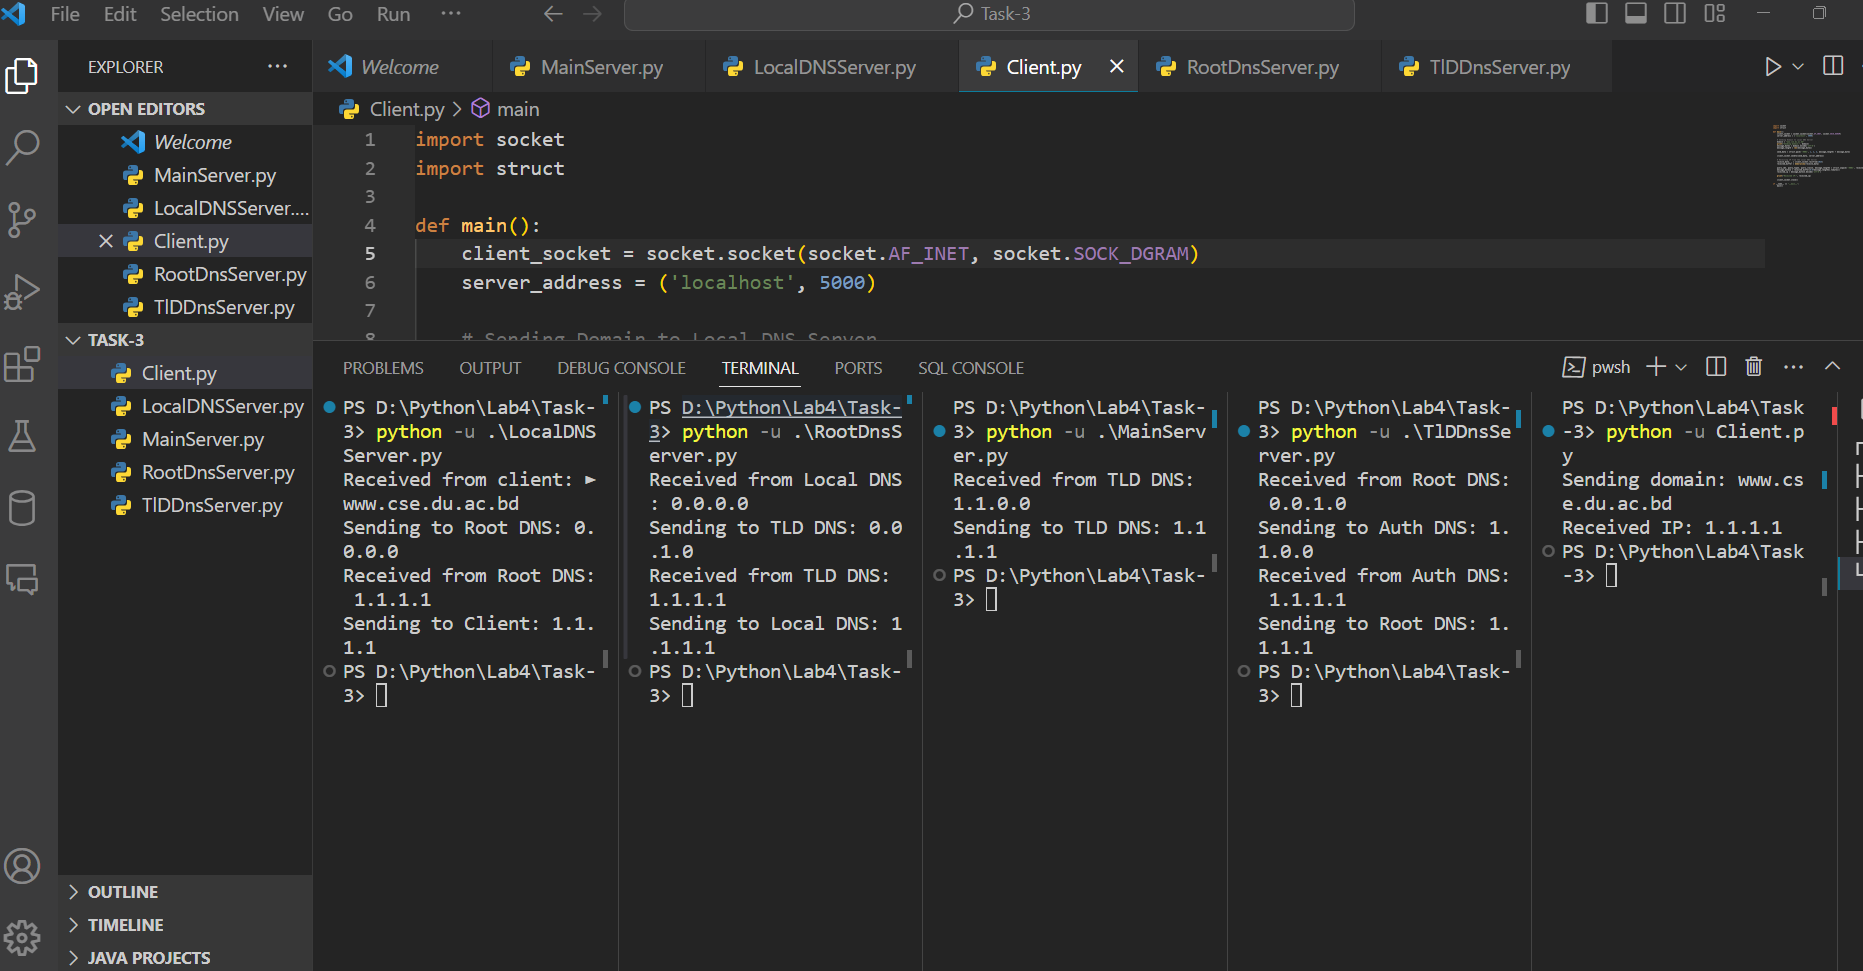
\includegraphics[width=0.8\textwidth]{result.png}
        \caption{Result}
        \label{fig:2}
    \end{figure}
    
    

\end{itemize}





\newpage
\section{Experience}
\begin{enumerate}
    \item  Configuring the DNS server to act as an authoritative server for a domain (e.g., cse.du.ac.bd) involves understanding and defining the necessary records (A, AAAA, CNAME, MX).
    \item We have create multiple server , thats why we needs more than one terminal 
    \item First we run all DNS server side program and then client request server for specific task
    \item Creating a tree of DNS servers with parent and child relationships provides a structured approach to DNS hierarchy.
    \item Ensuring the script accurately follows the DNS resolution path and retrieves the correct IP address may encounter challenges in parsing responses.
    \item Verifying the correct implementation of recursive DNS resolution requires monitoring the entire resolution process.
\end{enumerate}





\begin{thebibliography}{1}
  %\bibitem{book} Computer networking: a top-down approach 6th ed.
  \bibitem{DNS basic} DNS basic \url{- https://aws.amazon.com/route53/what-is-dns}
  \bibitem{Record types} Record types \url{- https://constellix.com/news/dns-record-types}
  \bibitem{geeksforgeeks} Domain Name System: \url{https://www.geeksforgeeks.org/domain-name-system-dns-in-application-layer/}
  \bibitem{youtube} DNS: \url{https://www.youtube.com/watch?v=mpQZVYPuDGU}
 \bibitem{Medium} Concept:\url{https://medium.com/@sureshpodeti/dns-domain-name-server-b000573e7dbe}
  

 
\end{thebibliography}



\end{document}

